%\RequirePackage{lineno}
\documentclass[aps,prc,preprint,superscriptaddress,showpacs,showkeys]{revtex4-1}
\usepackage{graphicx}
\begin{document}
\newcommand{\Jpsi}{J/\psi}
\newcommand{\pT}{p_{T}}

%\linenumbers
\title{{\Large Quarkonia suppression in PbPb collisions at $\sqrt s_{NN}$ =  2.76 TeV }}
\author{\large Vineet Kumar}
\author{\large Prashant Shukla}
\email{pshukla@barc.gov.in}
\affiliation{Nuclear Physics Division, Bhabha Atomic Research Center, Mumbai, India}
\affiliation{Homi Bhabha National Institute, Anushakti Nagar, Mumbai, India}
\author{\large Ramona Vogt}
\affiliation{Physics Division, Lawrence Livermore National Laboratory, Livermore, CA 94551, USA}
\date{\today}

\begin{abstract}
  We estimate the modification of quarkonia yields due to different processes 
in the medium produced in PbPb collisions at LHC energy. The quarkonia and heavy flavour 
cross sections calculated upto NLO are used in the study and shadowing corrections are obtained 
by EPS09 parameterization.
 A kinetic model is employed which incorporates quarkonia suppression inside QGP, suppression 
due to hadronic comovers and regeneration from charm pairs.
 Quarkonia dissociation cross section due to gluon collisions has been considered and
the regeneration rate has been obtained using the principle of detailed balance.
The modification in quakonia yields due to collisions with hadronic comovers has been estimated 
assuming it to be caused by pion.  
  The menifestations of these effects in different kinematic regions in
the nuclear modification factors for both $\Jpsi$ and $\Upsilon$ has been demonstrated
for PbPb collisions at $\sqrt s_{NN}$ =  2.76 TeV in comparison with the measurements.
  Both the suppression and regeneration due to deconfined medium strongly affect 
low intermediate $\pT$ range. The large observed suppression of $\Jpsi$ at $p_T$ 
above 10 GeV/$c$ exceeds the estimates of suppression by deconfined medium.
\end{abstract}

\pacs{12.38.Mh, 24.85.+p, 25.75.-q}
\keywords{quark-gluon plasma, quarkonia, suppression, regeneration}
\maketitle

%%%%%%%%%%%%%%%%%%%%%%%%%%%%%%%%%%%%%%%%%%%%%%%%%%%%%%%%%%%%%%%%%%%%%%%%%%%%%%%%%%%%%%%%%%%%%%%%%%%%%%%%%%%%%%%%%
\section{Introduction}
  Heavy ion collisions at relativistic energies are performed to create and characterize 
Quark Gluon plasma (QGP), a phase of strongly interacting matter at high energy density 
where quarks and gluons are no longer bound within hadrons. 
  Quarkonia state ($\Jpsi$ and $\Upsilon$) have been one of the most popular tools 
since their suppression was proposed as a signal of QGP \cite{Matsui:1986dk}.
  The understanding of these probes has evolved substantially via measurements 
through three generations of experiments: SPS (at CERN), RHIC (at BNL) and the LHC (at CERN) 
and by voluminous theoretical activities [For recent reviews see 
Refs.~\cite{Schukraft:2013wba,Kluberg:2009wc,Brambilla:2010cs}].
Quarkonia are produced early in the heavy ion collisions and if they evolve
through deconfined medium their yields should be suppressed in comparison with those in $pp$. 
 The first such measurement was the 'anomalous' $\Jpsi$ suppression discovered at the SPS 
which was considered as a hint of QGP formation. The RHIC measurements showed almost the 
same suppression at a much higher energy contrary to the expectation \cite{Brambilla:2010cs,Adare:2011yf}. 
 Such an observation was consistent with the scenarios that at higher collision energy the 
expected more suppression is compensated by regeneration of $\Jpsi$ by recombination of two 
independently produced charm quarks~\cite{Andronic:2003zv}.
After the LHC started PbPb collisions at $\sqrt s_{NN} = 2.76$ TeV, a wealth of
results have become available on quarkonia production \cite{Muller:2012zq,P.ShuklaforCMS:2014vna}. 
  The CMS experiment carries out $\Jpsi$ measurement at high transverse momentum 
($p_T>6.5$ GeV/$c$). The nuclear modification factor  $R_{AA}$ of these high $p_T$ 
prompt $\Jpsi$ decreases with increasing centrality \cite{Chatrchyan:2012np,Mironov:2013jaa} showing
moderate suppression even in the most peripheral collisions. 
  Moreover $R_{AA}$ is found to be nearly independent of $p_T$ (above 6.5 GeV$/c$) showing 
that $\Jpsi$ remain suppressed even at very high $p_T$ upto 16 GeV/$c$.
 On comparing with the STAR results \cite{Tang:2011kr} at RHIC it follows that the suppression of
(high $p_T$) $\Jpsi$ has increased with collision energy.
  The ALICE results \cite{Abelev:2013ila} of $\Jpsi$ covers low $p_T$ range which
have little or no centrality dependence. The ALICE $\Jpsi$ suppression decrease 
substantially with decreasing $p_T$ and at very low $p_T$ the suppression is small.
  When compared with PHENIX forward rapidity measurement at 
RHIC \cite{Adare:2011yf}, it suggests that low p$_T$ $\Jpsi$ are less suppressed at LHC.
 These observations suggest regeneration of $\Jpsi$ at low $p_T$ by 
recombination of independently produced charm pairs.
  The CMS measurements \cite{Chatrchyan:2011pe,Chatrchyan:2012lxa} reveal that 
the higher $\Upsilon$ states are more suppressed relative to the ground state, 
a phenomenon known as sequential suppression. The ALICE
 measurements in forward rapidity ($2.5 \leq y^{\Upsilon} \leq 4.0$) are 
consistent with CMS measurements in mid rapidity region ($|y^{\Upsilon}|\,\leq 2.4$).

 Many theoertical frameworks have been developed in pre-LHC years for the modification of 
quarkonia due to different processes. 
 The suppression of quarkonia in QGP are understood in terms of colour screening models  
e.g. Ref. \cite{Matsui:1986dk,Abdulsalam:2012bw}and alternatively in terms of dissociation of quarkonia 
by gluon collision process \cite{Bhanot:1979vb,Xu:1995eb}. The statistical models \cite{Andronic:2003zv,Andronic:2012dm}
offer estimates of the regeneration of quarkonia from charm quark pairs.
The inverse of gluon dissociation process is also used to estimate regeneration \cite{Thews:2000rj}.  
  The quarkonia yields in heavy ion collisions are also modified due to non-QGP effects such as
shadowing, an effect due to change of the parton distribution functions inside the nucleus,
and dissociation due to hadronic or comover interaction \cite{Vogt:2010aa}.
 There have been many recent calculations to explain the LHC results on quarkonia using a 
combination of above theoretical frameworks and models \cite{Zhao:2011cv,Emerick:2011xu}. 

In this paper, we calculate the quarkonia (both $\Jpsi$ and $\Upsilon$) production and
suppression in a kinetic model which includes dissociation due to thermal gluons, modification 
of yield due to change in parton distribution functions inside nucleus and due to collisions with 
comover hadrons. Regeneration by thermal heavy quark pairs is also take into account. 
 Our goal is obtain the nuclear modification factor of quarkonia as a function of transverse 
momentum and centrality of collision to be compared with experimental data from CMS 
and ALICE.

\section{The production rates and shadowing}
The production cross sections for heavy quark pairs are calculated to NLO in pQCD  
using the CTEQ6M parton densities \cite{Pumplin:2002vw,Pumplin:2000vx}.  The central EPS09 parameter set 
\cite{Eskola:2009uj} is used to calculate the modifications of the parton densities in 
PbPb collisions.  We use the same set of parameters
as that of Ref.~\cite{Cacciari:2005rk} with the NLO calculation of Ref.~\cite{Mangano:1991jk}
to obtain the exclusive $Q \overline Q$ pair rates.  
 The production cross sections for heavy flavor and quarkonia at $\sqrt{s_{_{NN}}}= 2.76$ 
TeV \cite{Kumar:2012qx} are given in Table~\ref{NLOcros}.  The number of $Q \overline Q$ pairs
in a minimum bias PbPb event is obtained from the per nucleon cross
section, $\sigma_{\rm PbPb}$, by
\begin{eqnarray}
N_{Q \overline Q} = {A^2 \sigma_{\rm PbPb}^{Q \overline Q}  \over  
\sigma_{\rm PbPb}^{\rm tot}} \, \, .
\end{eqnarray}
 At 2.76 TeV, the total PbPb cross section, $\sigma_{\rm PbPb}^{\rm tot}$, 
is 7.65 b \cite{Chatrchyan:2011sx}.

\begin{table}
\caption[]{Heavy quark and quarkonia production  cross sections at
$\sqrt{s_{_{NN}}}= 2.76$ TeV. The cross sections are given per nucleon pair while
$N^{\rm PbPb}$ (including shadowing) gives the number of heavy quark pair/quarkonia per PbPb event.}
\label{NLOcros}
\begin{tabular}{l|l|l|l|l} 
\hline 
\hline
             & $ c \overline c$       &$\Jpsi$       & $ b \overline b$        & $\Upsilon$   \\              
\hline
$\sigma_{\rm PbPb}$ & $1.76^{+2.32}_{-1.29}$ mb  & 31.4 $\mu$b   & $89.3^{+42.7}_{-27.2} \mu$b  & 0.38 $\mu$b  \\
$N^{\rm PbPb}$     & $9.95^{+13.10}_{-7.30}$     & $0.177$       & $0.50^{+0.25}_{-0.15}$       & $0.01$       \\
$N^{pp}$          &                         & $0.177/0.93$  &                        & $0.01/0.95$   \\
\hline
\hline
\end{tabular}
\end{table}





%%%%%%%%%%%%%%%%%%%%%%%%%%%%%%%%%%%%%%%%%%%%%%%%%%%%%%%%%%%%%%%%%%%%%%%%%%%%%%%%%%%%%%%%%%
\section{Modification of quarkonia in the presence of QGP}
 In the kinetic approach \cite{Thews:2000rj}, the proper time ($\tau$) evolution of the quarkonia 
population $N_{QO}$
is given by the rate equation 

\begin{equation}\label{eqkin}
{dN_{QO} \over d\tau}  =  - \lambda_D  \rho_g N_{QO} + \lambda_F {N_{Q \bar{Q}}^{2} \over V(\tau)},
\end{equation}
where $V(\tau)$ is the volume of the deconfined spatial region and $N_{Q \bar{Q}}$ is the number of initial 
heavy quark pairs produced per event depending on the centrality ($N_{\rm part}$).
 The $\lambda_{D}$ is the dissociation rate obtained by the dissociation cross-section averaged over the momentum 
distribution of gluons and $\lambda_{F}$ is the formation rate obtained by the formation cross-section 
averaged over the momentum distribution of $Q$ and $\bar Q$. $\rho_g$ is the density of thermal gluons.
 The number of quarkonia at freeze-out time $\tau_f$ is given by solution of Eq.~(\ref{eqkin}) as
\begin{equation}
N_{QO}(p_T) = S(p_T) \,N_{QO}^{\rm PbPb}(p_T)+N_{QO}^F(p_T).
\label{eqbeta}
\end{equation}
Here $N_{QO}^{0}(p_T)$ is the number of initially produced quarkonia (including shadowing) as a function 
of $p_T$ and $S(p_T)$ is their survival probability from gluon collisions at freeze-out time $\tau_f$ and 
is written as
\begin{equation}
S(\tau_f,p_T) = \exp \left( {-\int_{\tau_0}^{\tau_f}f(\tau) \lambda_{\rm D}(T,p_T)\,\rho_g(T)\,d\tau} \right).
\end{equation}
 The temperature $T(\tau)$ and the QGP fraction $f(\tau)$ evolve from initial time $\tau_0$ 
to freeze-out time $\tau_f$ due to expansion of QGP. The initial temperatures and thus the 
evolution is dependent on $N_{\rm part}$.
$N_{QO}^F(p_T)$ is the number of regenerated quarkonia per event and is given by
\begin{equation}
N_{QO}^F(p_T)=S(\tau_f,p_T)N_{Q \bar{Q}}^{2} \int_{\tau_0}^{\tau_f}{{\lambda_{\mathrm{F}}(T,p_T) \over V(\tau)\,S(\tau,p_T)} d\tau}
\end{equation}

   The nuclear modification factor ($R_{AA}$) can be written as 
\begin{equation}
R_{AA}(p_T)=S(p_T) \, R(p_T) + \frac{N_{QO}^F(p_T)}{N_{QO}^{pp}(p_T)}.
\label{raa}
\end{equation}
Here $R(p_T)$ is the shadowing factor.
$R_{AA}$ as a function of collision centrality, including the regeneration will be  
\begin{equation}
R_{AA}(N_{\rm part}) = \frac{\int_{p_{T\,\rm Cut}} N_{QO}^{pp}(p_T)S(p_T)\, R(p_T) dp_T}{\int_{p_{T\,\rm Cut}} N_{QO}^{pp}(p_T) dp_T} + 
\frac{\int_{p_{T\, \rm Cut}} N_{QO}^F(p_T) dp_T}{\int_{p_{T\, \rm Cut}} N_{QO}^{pp}(p_T) dp_T}
\label{raa2}
\end{equation}
Here $p_{\rm Cut}$ defines the $p_T$ range as per the experimental measurements.
 $N_{QO}^{pp}(p_T)$ is the unmodified $p_T$ distribution of quarkonia obtained by NLO 
calculations which is scaled to a particular centrality of PbPb collisions.

  The evolution of the system for each centrality of collision is governed by
an isentropical cylindrical expansion with volume element
\begin{equation}
V(\tau) = \tau\,\pi\,(R + {1\over 2} a \, \tau^2 )^{2},
\end{equation}
 where a$_T$=0.1c$^2$ fm$^{-1}$ is the transverse acceleration \cite{Zhao:2011cv}.
 The initial transverse size, $R$ as a function of centrality is obtained as 
\begin{equation}
R(N_{\rm part}) = R_{0-5\%} \, \sqrt{N_{\rm part} \over (N_{\rm part})_{0-5\%} },
\label{RVsNPart}
\end{equation}
where $R_{0-5\%} = 0.92\,R_{\rm Pb}$; $R_{\rm Pb}$ being the radius of the Pb nucleus.

  The evolution of entropy density for each centrality is obtained by entropy conservation 
condition $s(T)\,V(\tau)= s(T_0)\,V(\tau_0)$.
 The equation of state obtained by Lattice QCD along with hadronic resonance gas \cite{Huovinen:2009yb} 
is used for $s(T)$ to obtain the temperature as a function of proper time $\tau$.
  The initial entropy density for each centrality is calculated using 
\begin{equation}
s(\tau_0) = s(\tau_0)|_{0-5\%} \left(\frac{dN/d\eta}{N_{\rm part}/2}\right)/\left(\frac{dN/d\eta}{N_{\rm part}/2}\right)_{0-5\%}.
\label{TempNpart}
\end{equation}
  Measured values of $\left(\frac{dN/d\eta}{N_{\rm part}/2}\right)$ as a function of $N_{\rm part}$ 
\cite{Aamodt:2010cz} are used in the calculations.
 The initial entropy density $s(\tau_0)|_{0-5\%}$ for 0-5\% centrality is obtained as 
\begin{eqnarray}
s(\tau_0)|_{0-5\%}  = {a_{\rm m} \over V(\tau_0)|_{0-5\%}}   \left(\frac{dN}{d\eta}\right)_{0-5\%} . 
\label{TempVsMult}
\end{eqnarray}  
 Here $a_m=5$ relating the total entropy with the mutliplicity is obtained from 
hydrodynamic calculations \cite{Shuryak:1992wc}. 

Using $(dN/d\eta)_{0-5\%}$=1.5$\times$1600 obtained from the charge particle multiplicity measured 
in PbPb collisions at 2.76 TeV and with lattice
equation of state we obtain the initial temperature for the most central collisions 
as 0.492 GeV at time $\tau_0$ = 0.3 fm/c.

The (proper)time evolution of temperature is shown in Fig.~\ref{fig:TauVsTemp}(a) 
and QGP fraction in Fig.~\ref{fig:TauVsTemp}(b) in case of most central (0-5$\%$) collisions
for both longitudinal and cylindrical expansions using first order and lattice Equation of 
state (EOS). 
 For the first order EOS, $T_C$ = 0.170 GeV and the QGP fraction goes from 1 to 0 at this
temperature assuming a mixed phase of QGP and hadrons.
  The QGP fraction in case of lattice EOS governs number of degrees of freedom 
decided by entropy density. It is fixed to 1 above an entropy density 
corresponding to a 2-flavour QGP and fixed to zero below entropy density for a hot 
rasonance gas. The freeze out temperature in all cases is $T_f=0.140$ GeV.  


\begin{figure}
\includegraphics[width=0.49\textwidth]{Figures/Fig1a_TauVsTemp.eps}
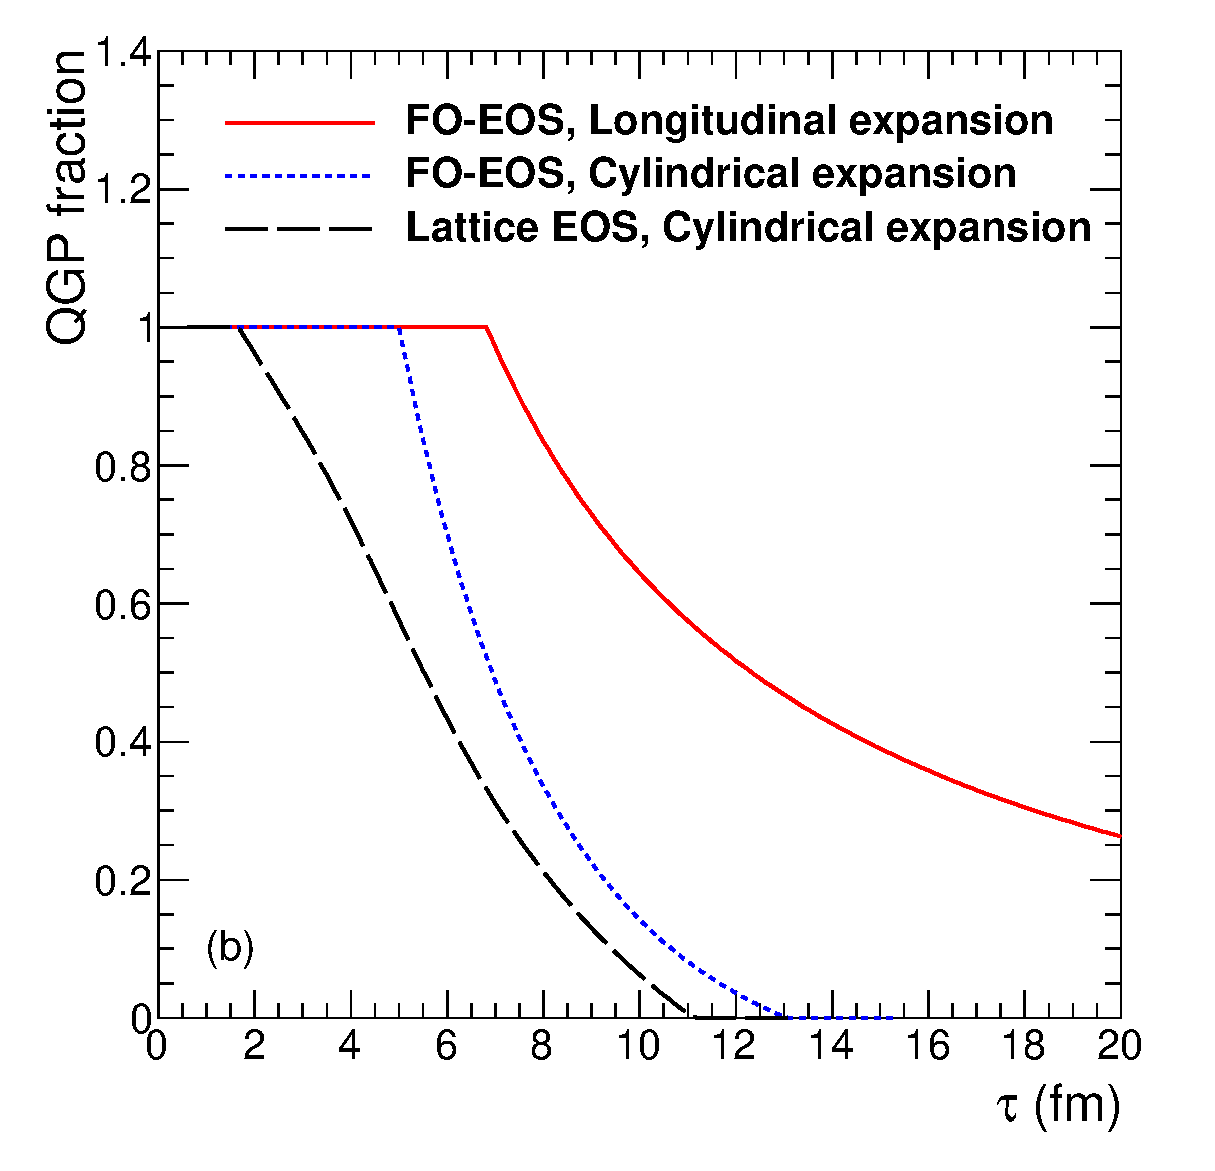
\includegraphics[width=0.49\textwidth]{Figures/Fig1b_TauVsFQGP.eps}
\caption{(Color online) (a) Temperature and (b) QGP fraction in the system as a function of proper 
time $\tau$ in case of the most central (0-5$\%$) collisions for longitudinal and cylindrical expansions 
using first order and lattice equation of state . }
\label{fig:TauVsTemp}
\end{figure}

%%%%%%%%%%%%%%%%%%%%%%%%%%%%%%%%%%%%%%%%%%%%%%%%%%%%%%%%%%%%%%%%%%%%%%%%%%%%%%%%%%%%%%%%%%%%%%%%%




%\begin{table}
%\caption[]{Quarkonia properties as predicted by non-relativistic potential model using 
%``Cornell'' potential \cite{Karsch:1987pv}.}
%\label{Tab:QuarkoniaProperties}
%\begin{tabular}{l|l|l|l|l|l|l|l|l} 
%\hline   
%\hline
%    &$\Jpsi$  &$\chi_c$  &$\psi(2S)$ &$\Upsilon(1S)$ &$\chi_b(1P)$ &$\Upsilon(2S)$ &$\chi_b(2P)$ &$\Upsilon(3S)$ \\ 
%\hline 
%Mass [GeV/$c^2$]                      &3.10     &3.53  &3.68  &9.46  &9.99  &10.02  &10.26   &10.36 \\
%Binding Energy $\epsilon_{0}$ [GeV]                  &0.64     &0.20  &0.05  &1.10  &0.67  &0.54   &0.31    &0.20 \\
%%Radius [fm]                           &0.25     &0.36  &0.45  &0.14  &0.22  &0.28   &0.34    &0.39 \\
%%Formation time $\tau_{\rm Form}$ [fm]    &0.89     &2.0   &1.5   &0.76  &2.6   &1.9    &2.6      &2.4 \\
%\hline
%\hline
%\end{tabular}
%\end{table}



\subsection{Dissociation Rate}
   In colour dipole approximation the gluon dissociation cross section as function of gluon energy $q^0$
in the quarkonium rest frame is given by \cite{Bhanot:1979vb}
\begin{equation}
\sigma_{D}(q^{0}) = {8\pi \over 3} \, {16^2 \over 3^2} {a_0 \over m_Q}  \frac{(q^0/\epsilon_0 - 1)^{3/2}} {q^0/\epsilon_0^5},
\end{equation}
 where $\epsilon_0$ is the quarkonia binding energy and $m_Q$ is the charm/bottom quark mass 
and $a_0=1/\sqrt{m_Q\epsilon_0}$.
The values of $\epsilon_0$ are taken as 0.64 and 1.10 GeV for ground states $\Jpsi$ and $\Upsilon(1S)$,
respectively \cite{Karsch:1987pv}. For excited states of bottommonia we use dissociation
cross section from Ref.~\cite{Arleo:2001mp}.

 Figure \ref{fig:SigmaDQ0} shows the gluon dissociation cross section of $\Jpsi$ and $\Upsilon(1S)$
as a function of gluon energy. 
 The dissociation cross section is zero when gluon energy is less than the binding energy
of the quarkonia. It increases with gluon energy and reaches  maximum at 1.2 (1.5) GeV for 
$\Jpsi\,(\Upsilon)$. At higher gluon energy, the interaction probability decreases.
$q^0$ is related to the centre of mass energy square $s$, of quakonium-gluon system as
\begin{eqnarray}
 q^{0} = \frac{s-M_{QO}^{2}}{2\,M_{QO}}.
\end{eqnarray}  
  Using this relation, $\sigma_{D}(q^0(s))$ can be obtained which we write as $\sigma_{D}(s)$.
The $s$ can be obtained as
$s=M_{QO}^{2} + 2  p_g \, \sqrt{M_{QO}^2 + p^2} (1-{\rm cos\theta})$,
where $M_{QO}$ and $p$ are mass and momentum of quarkonium and $\theta$ is its
angle with gluon.
 
 We can calculate dissociation rate as a function of quarkonium momentum 
by integrating the dissociation cross-section on thermal gluon momentum 
distribution $f_{g}(p_g)$ as   
\begin{eqnarray}
\lambda_{D} \rho_{g}  & = & \langle \sigma v_{\rm rel} \rangle \,\rho_{g}  = 
      \frac{g_g}{(2\pi)^{3}} \int d^{3}p_g \, f_{g}(p_g)  \, \sigma_{D}(s) v_{\rm rel}(s)  \nonumber \\ 
& = &\frac{g_g}{(2\pi)^{3}} \int  2\pi p_g^{2} dp_g f_{g}(p_g) \int \sigma_{D}(s) v_{\rm rel}(s) d({\rm cos\theta})  
\end{eqnarray}
 The relative velocity $v_{\rm rel}$ between the quarkonium and the gluon is given by
\begin{eqnarray}
 v_{\rm rel}  = {s- M_{QO}^{2} \over 2  p_g\, p_g\sqrt{M_{QO}^2 + p^2} }  
\label{eq7}
\end{eqnarray}

  The gluon dissociation rates of $\Jpsi$ as a function of temperature are shown in 
Fig.~\ref{fig:DRateVsTempAndPt}(a) and as a function of transverse momentum are
 shown in Fig.~\ref{fig:DRateVsTempAndPt}(b).
The dissociation rate increases with temperature due to increase in gluon density. 
Dissociation rate of quarkonium is maximum when it is at rest and decreases with 
its (transverse) momentum.


\begin{figure}
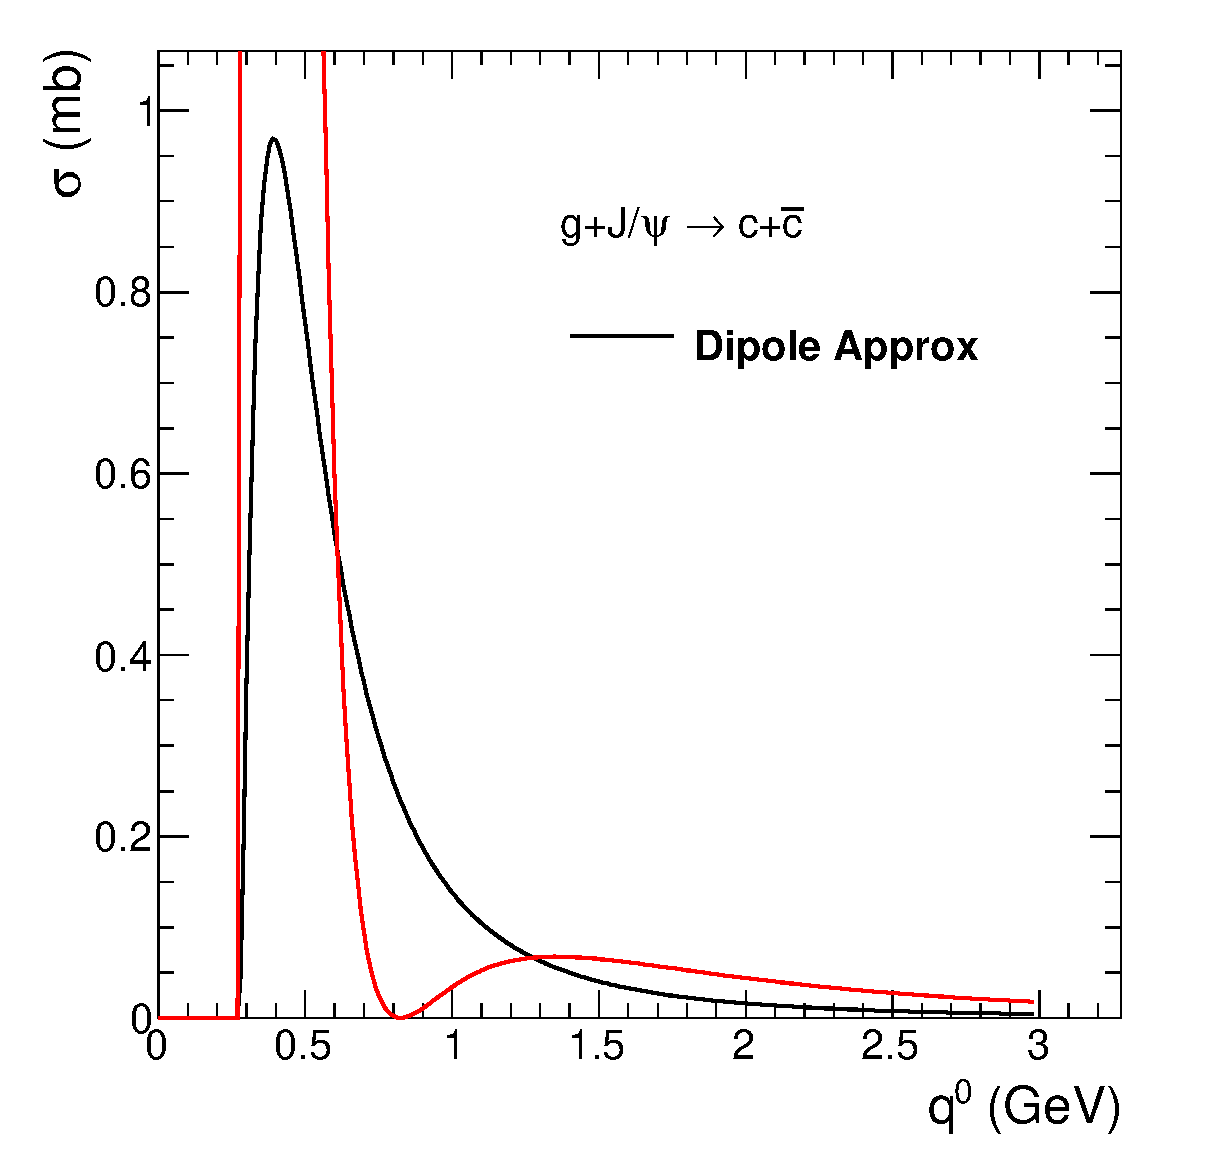
\includegraphics[width=0.60\textwidth]{Figures/Fig2_SigmaDq0.eps}
\caption{Gluon dissociation cross-section of quarkonia as a function of gluon energy ($q^{0}$) in
quarkonia rest frame.}
\label{fig:SigmaDQ0}
\end{figure}

\begin{figure}
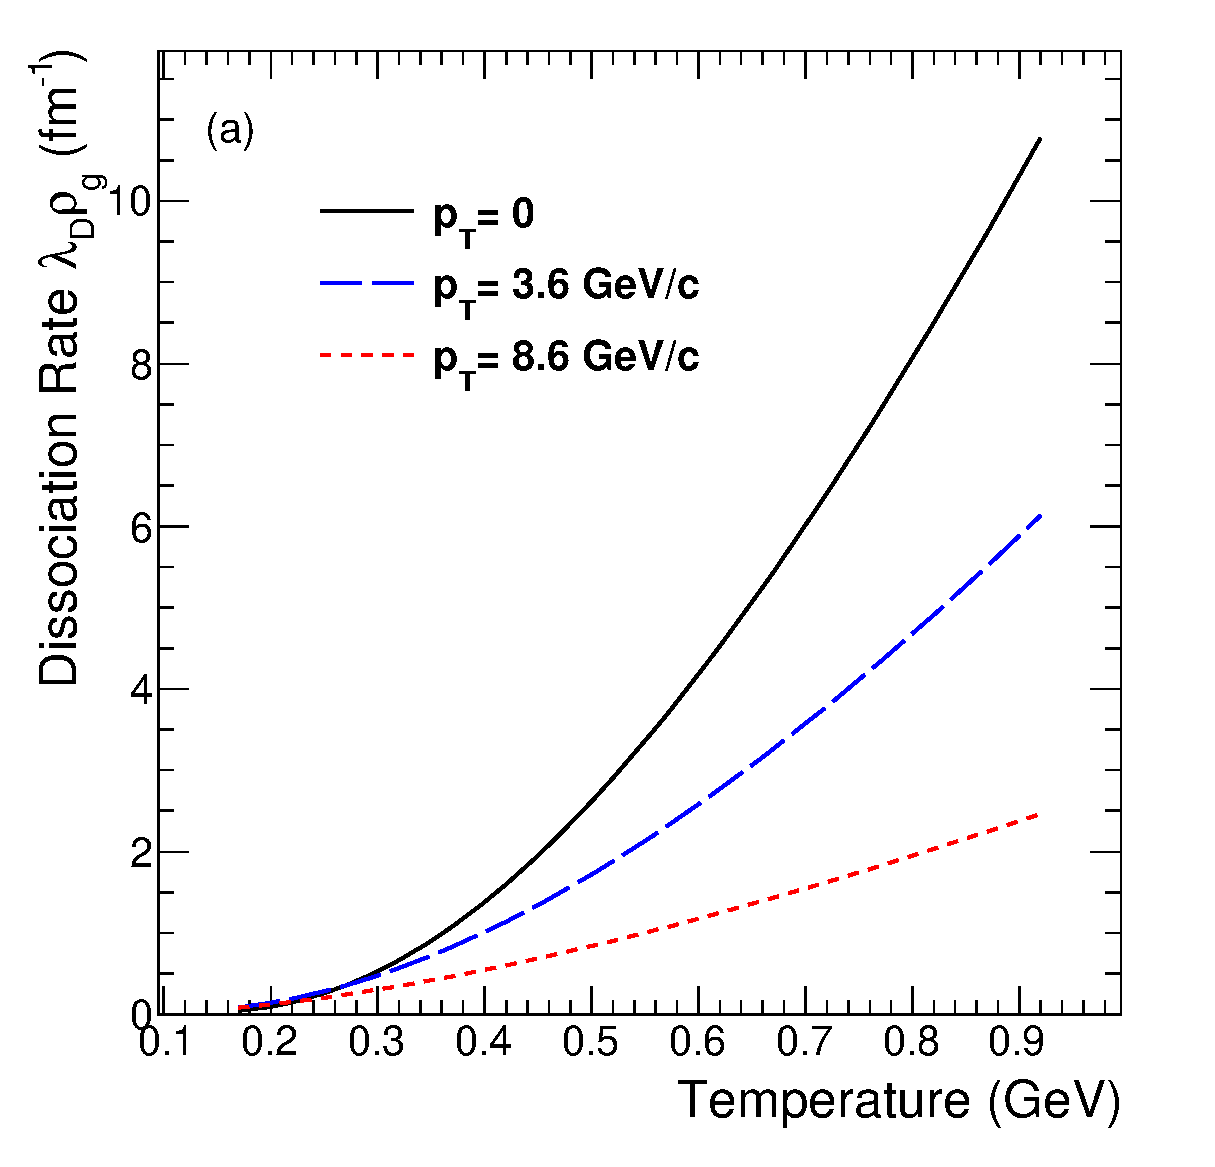
\includegraphics[width=0.49\textwidth]{Figures/Fig3a_DRateVsT.eps}
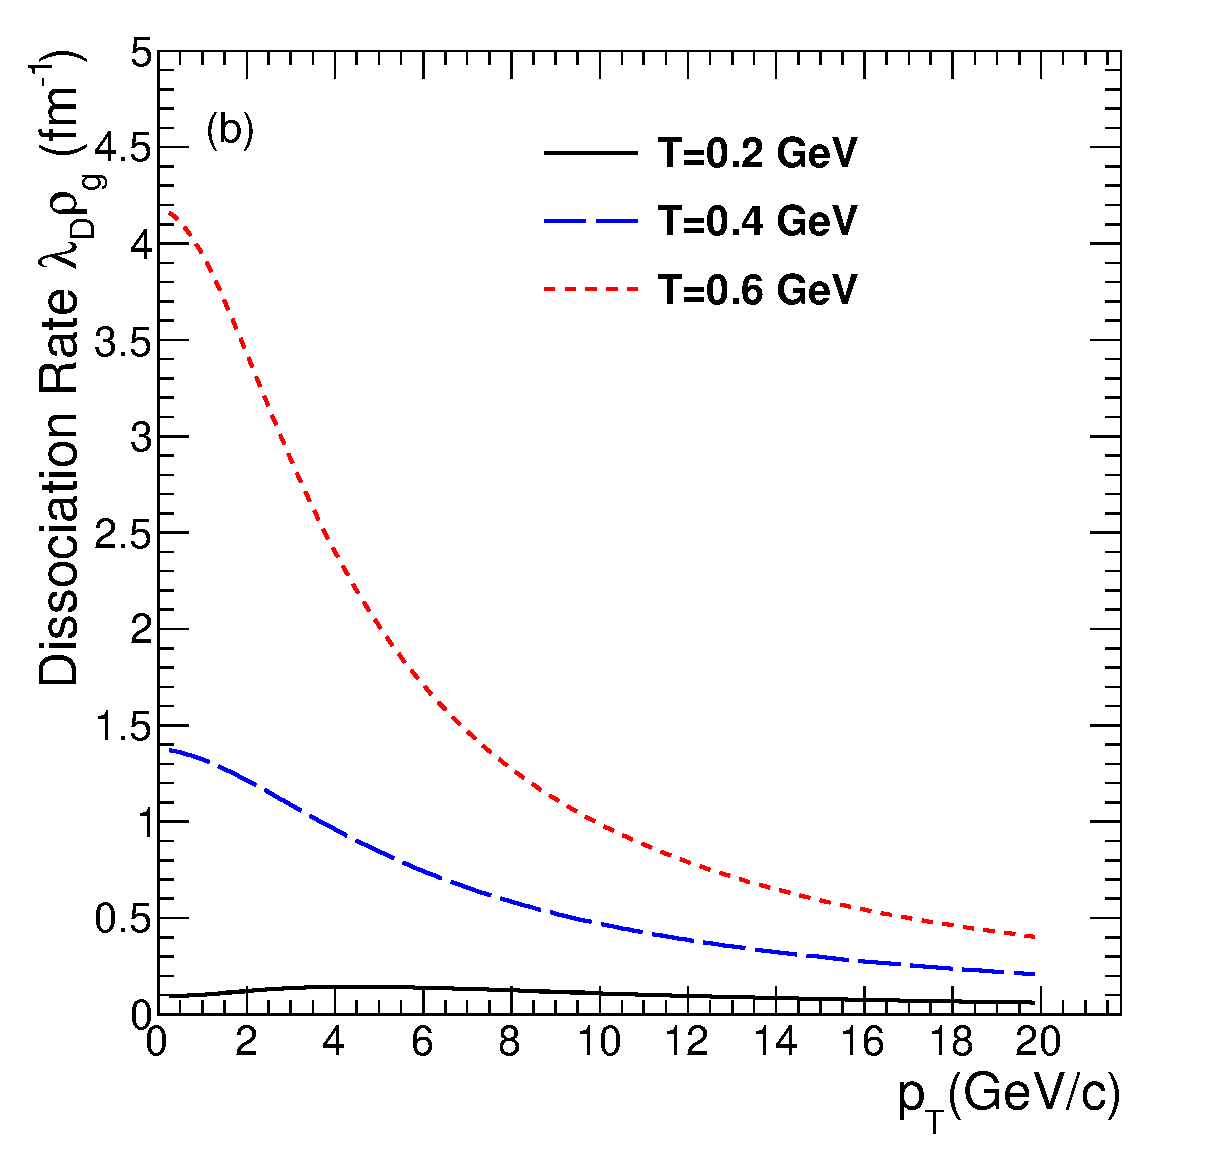
\includegraphics[width=0.49\textwidth]{Figures/Fig3b_DRateVsPt.eps}
\caption{(Color online) Gluon dissociation rate of $\Jpsi$ as a function of (a) temperature and  
(b) as a function of transverse momentum.}
\label{fig:DRateVsTempAndPt}
\end{figure}


%
%and $q^0$ the gluon energy in the $J/ \psi$ rest frame is related to centre of mass 
%energy of $\Jpsi$-gluon system as
%\begin{eqnarray}
% q^{0} = \frac{s-M_{\Jpsi}^{2}}{2\,M_{\Jpsi}},
%\end{eqnarray}

%%%%%%%%%%%%%%%%%%%%%%%%%%%%%%%%%%%%%%%%%%%%%%%%%%%%%%%%%%%%%%%%%%%%
%%%%%%%%%%%%%%%%%%%%%%%%%%%%%%%%%%%%%%%%%%%%%%%%%%%%%%%%%%%%%%%%%%
%`If we consider that the $J/ \psi$ moves in the transverse direction with a four-velocity
%$u=(M_T, \vec{P_T}, 0)/M_{\Jpsi}$, where $M_T=\sqrt{p_T^2+M^2_{J/ \psi}}$ is defined as the $\Jpsi$'s
%transverse mass. 
%A gluon with a four-momentum $k=(k^0,\vec{k})$
%in the rest frame of the parton gas has an energy $q^0=k\cdot u$
%in the rest frame of the $\Jpsi$ given by
%\begin{eqnarray}
% q^{0} &= &\frac{k^{0}\,m_{T} + \vec{k} \cdot \vec{p_{T}}}{M_{\Jpsi}}, \nonumber \\
%       &= &\frac{s-M_{\Jpsi}^{2}}{2\,M_{\Jpsi}},
%\end{eqnarray}
%The dissociation rate is given by 
%\begin{eqnarray}
%\lambda_D = \langle v_{\rm rel} \sigma_{D} (k \cdot u)\rangle_k &= &\frac{\int d^3k v_{\rm rel} \sigma_{D} (k \cdot u) f(k^0,T)}{\int d^3k f(k^0,T)},
% \label{eq5}
%\end{eqnarray}
%where the gluon distribution in the rest frame of the parton gas is
%\begin{equation}
%  f(k^0,T)=\frac{\lambda_g(=16)}{e^{k^0/T}-1} \label{eq6}.
%\end{equation}
%The relative velocity $v_{\rm rel}$ between the $\Jpsi$ and a gluon is
%\begin{eqnarray}
% v_{\rm rel}  =  \frac{P_{\Jpsi}\cdot k}{k^0M_T} \,\,
%              =  1-\frac{\vec{k}\cdot\vec{P}_T}{k^0M_T} \,\,
%              =  {s- M_{\Jpsi} \over 2E_1E_2}  
%\label{eq7}
%\end{eqnarray}
%Changing the variable to the gluon momentum, $q=(q^0,\vec{q})$, in
%the rest frame of the $\Jpsi$, and writing $\rho_g = \int d^3k f(k^0,T)$, 
%the Eq.~(\ref{eq5}) can be rewritten as
%\begin{eqnarray}
%\lambda_D \rho_g  =  \int d^3q \frac{M_{\Jpsi}}{m_T}\sigma_{D}(q^0) f(k^0,T).
%\label{eq8}
%\end{eqnarray}
%Using $ k^0=(q^0M_T+\vec{q}\cdot\vec{P}_T)/M_{\Jpsi}$ in Eq.~\ref{eq8} and solving
%\begin{eqnarray} 
%\lambda_D\,\rho_g &= &\frac{M_{\Jpsi}}{m_T} \int d^3q \, \sigma_{D}(q^0) \frac{\lambda_{g}} {  e^{ \frac{q^0m_{T}}{M_{\Jpsi}T}} e^{ \frac{ \vec{q}\cdot \vec{p_{T} } }{ M_{\Jpsi}T }  } -1}  \nonumber \\
%%&= &\frac{\lambda_{g}}{2\pi^3} \frac{M_{\Jpsi}}{m_T} \int d^3q \, \sigma_{D}(q^0)   \sum_{n=1}^{\infty}  e^{ \frac{-n\,q^0 m_{T}}{M_{\Jpsi}T}} e^{  \frac{-n\,\vec{q}\cdot \vec{p_{T}}}{M_{\Jpsi}T}}  \nonumber \\
%%&= &\frac{\lambda_{g}}{2\pi^3} \frac{M_{\Jpsi}}{m_T}  \sum_{n=1}^{\infty} 2\pi  \int (q^0)^2 dq^0 \, \sigma_{D}(q^0)\,e^{ \frac{-n\,q^0m_{T}}{M_{\Jpsi}T}}  \int_{1}^{-1} e^{  \frac{-n\,q^0\,p_{T} cos\theta}{M_{\Jpsi}T}} d(cos\theta) \nonumber \\
%%&= &\frac{\lambda_{g}}{2\pi^3} \frac{M_{\Jpsi}}{m_T} \sum_{n=1}^{\infty} 2\pi  \int (q^0)^2 dq^0 \, \sigma_{D}(q^0)\,e^{ \frac{-n\,q^0 m_{T}}{M_{\Jpsi}T}} 
%%    \left[ e^{-\frac{nq^0 p_T}{M_{\Jpsi}T}} - e^{\frac{nq^0 p_T}{M_{\Jpsi}T}} \right]\,\frac{M_{\Jpsi}T}{nq^0 p_T}  \nonumber \\
%&= &\frac{\lambda_{g}}{2\pi^3} \frac{M_{\Jpsi}^2}{m_T} 2\pi \sum_{n=1}^{\infty} \frac{T}{n} \int_{\epsilon_0}^{\infty} q^0 dq^0 \, \sigma_{D}(q^0)  
%     \,e^{ \frac{-n\,q^0 m_{T}}{M_{\Jpsi}T}} 
%     \frac{1}{p_T} \left[e^{\frac{n q^0 p_T}{M_{\Jpsi}T}} - e^{- \frac{n q^0 p_T}{M_{\Jpsi}T}}\right] \\ \nonumber
%\label{dissrate}
%\end{eqnarray}

%%%%%%%%%%%%%%%%%%%%%%%%%%%%%%%%%%%%%%%%%%%%%%%%%%%%%%%%%%%%%%%%%%%%
%%%%%%%%%%%%%%%%%%%%%%%%%%%%%%%%%%%%%%%%%%%%%%%%%%%%%%%%%%%%%%%%%%%%
% The special case of Eq.~(\ref{dissrate}) for J/$\psi \,p_T = 0$ is
%\begin{eqnarray} 
%  \frac{1}{p_T} \left[e^{\frac{n q^0 p_T}{M_{\Jpsi}T}} - e^{- \frac{n q^0 p_T}{M_{\Jpsi}T}}\right] = {2nq^0\over M_{\Jpsi}T}.
%\label{case}
%\end{eqnarray}
%Using this we get 
%\begin{eqnarray} 
% \lambda_D\,\rho_g &= &  4\pi \int (q^0)^2\,dq^0 \, \sigma_{D}(q^0) \frac{\lambda_{g}} {e^{\frac{q^0}{T}} -1}
%\end{eqnarray}
%%%%%%%%%%%%%%%%%%%%%%%%%%%%%%%%%%%%%%%%%%%%%%%%%%%%%%%%%%%%%%%%%%%%%%%%%%%%%%%%%%%%


\subsection{Formation Rate}
  We can calculate formation cross section from dissociation cross section using detailed balance 
relation \cite{Thews:2000rj,Thews:2005vj} as
\begin{equation}
\sigma_{F} = \frac{48}{36}\,\sigma_{D}(q^0)\frac{(s-M_{QO}^2)^{2}}{s(s-4m_Q^{2})}.
\end{equation}
The formation rate of quarkonium with momentum {\bf p} can be written as
\begin{equation}
d\lambda_{F}/d{\rm\bf p} = \int \sigma_{F}(s)\, v_{\rm rel}(s)\,f_{Q}(p_1)\, f_{\bar{Q}} (p_2) \,d^{3}p_1 \,d^{3}p_2 \, \delta({\rm\bf p}-( {\rm\bf p_1} + {\rm\bf p_2} ))
\end{equation}
  Here $f_{Q/\bar{Q}}(p)$ are taken as thermal distribution function of  $Q/\bar{Q}$ which are 
normalized to one as per $\int f_{Q}(p) d^{3}p  = 1 $.
$v_{\rm rel}$ is relative velocity between $Q\bar{Q}$ quark pair and is given by
\begin{eqnarray}
v_{\rm rel} &=& {\sqrt{(p_{1}.p_{2})^{2} - m_Q^{4} } \over E_{1} \, E_{2}} %\nonumber \\
%            &=& \frac{\sqrt{s(s-4m_Q^{2})}}{2E_1E_2}.
\end{eqnarray}
 Here $p_1 = (E_1,{\bf p_{1}})$, $p_{2} = (E_{2},{\bf p_{2}})$ are four momenta of heavy quark and 
anti-quarks, respectively.
% The centre of mass energy square of c$\bar{c}$ system is 
% $s =  2\,m_Q^{2} + 2 E_1E_2 - 2 |\vec{p_1}||\vec{p_2}|cos\theta$.

Figure \ref{fig:ForRateVsTempAndPt} (a) shows variation of formation rate of $\Jpsi$ as a funcion 
of medium temperature and Fig.~\ref{fig:ForRateVsTempAndPt} (b) shows as a function of transverse 
momentum of $\Jpsi$.
The $\Jpsi$ generated from recombination of uncorrelated heavy quark pairs will have 
softer $p_{T}$ distributions than that of $\Jpsi$ coming from initial hard scattering and thus 
effect of recombination will be important only at low $p_T$.

\begin{figure}
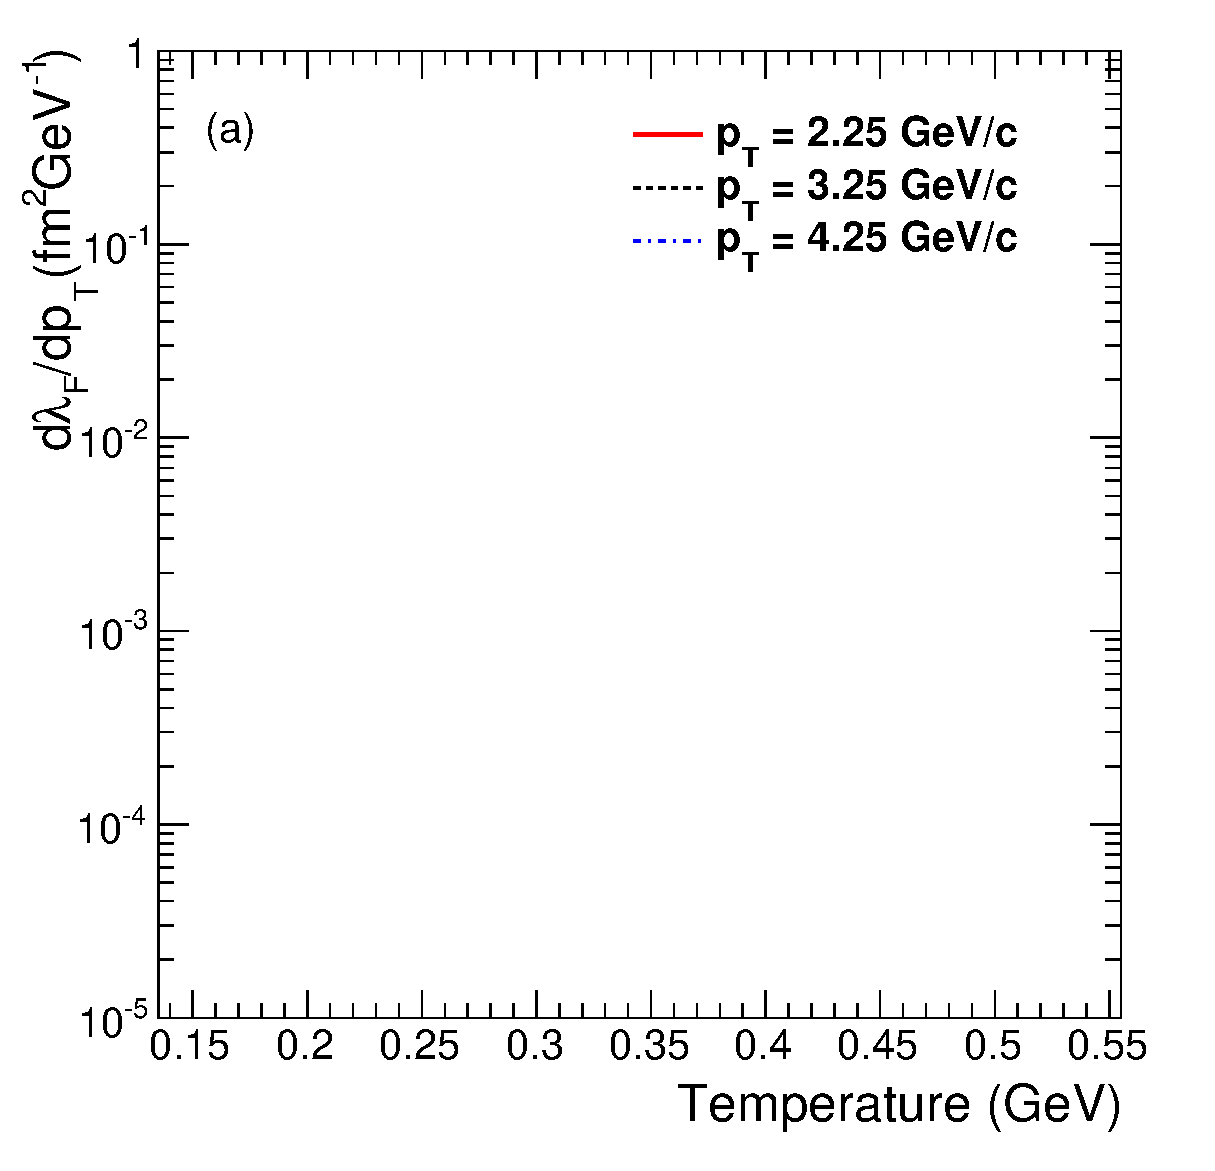
\includegraphics[width=0.49\textwidth]{Figures/Fig4a_FRateVsT.eps}
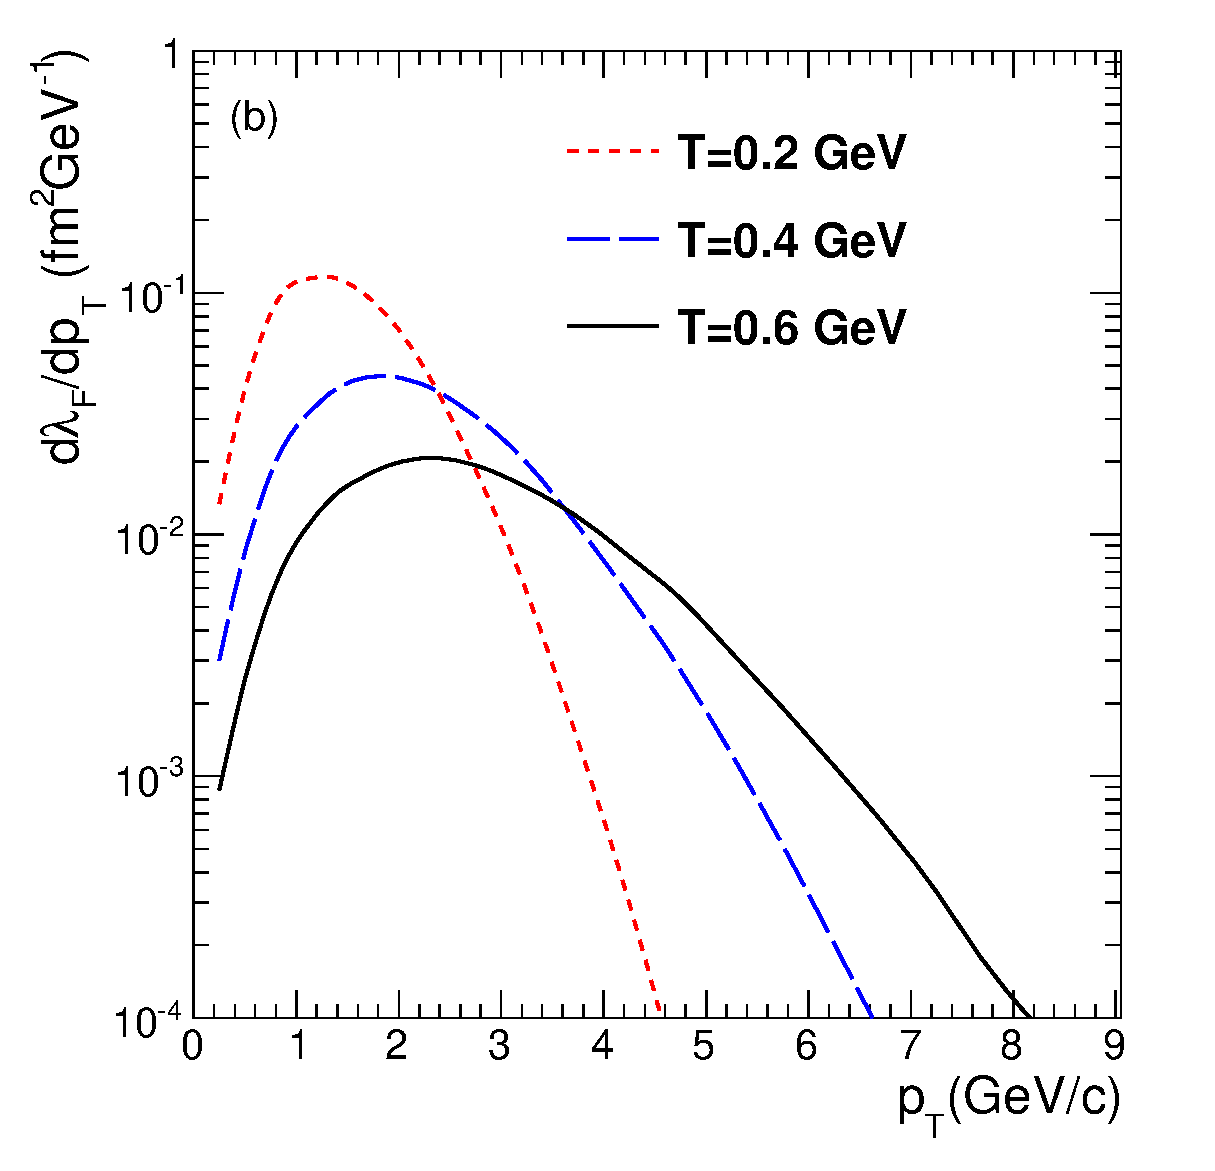
\includegraphics[width=0.49\textwidth]{Figures/Fig4b_FRateVsPt.eps}
\caption{(Color online) Formation rate of  $\Jpsi$ as (a) a function of  temperature and (b) as a 
function of transverse momentum.}
\label{fig:ForRateVsTempAndPt}
\end{figure}

%The formation and dissociation rates are shown for $\Jpsi$, we use same formalism to calculate
%these rates for $\Upsilon$ also.


\begin{figure}
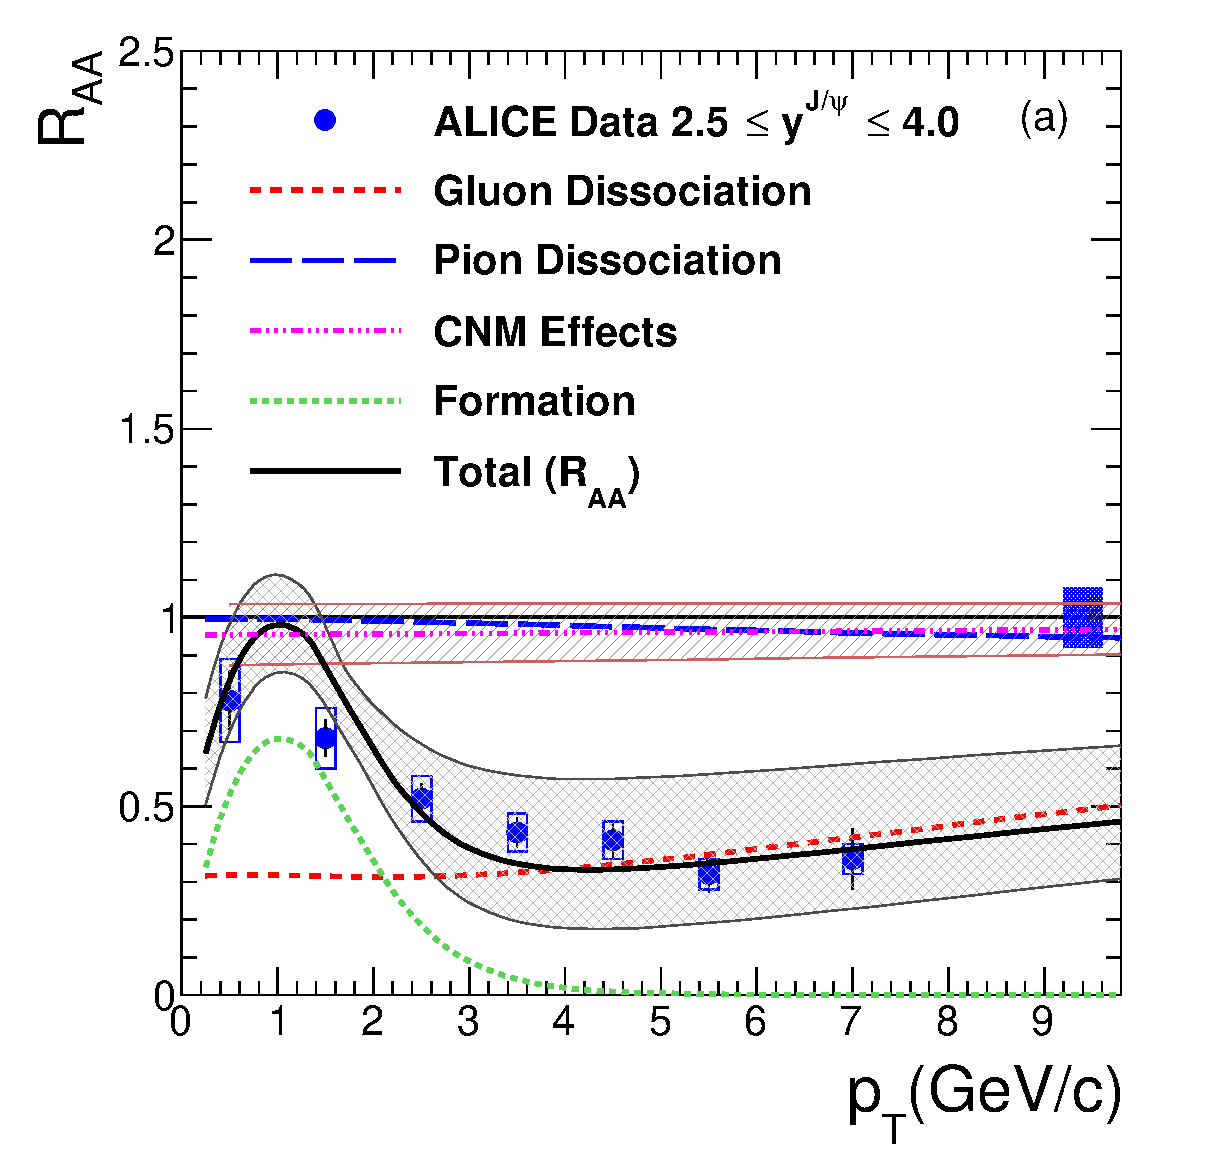
\includegraphics[width=0.49\textwidth]{Figures/Fig5a_ALICE_RAAPt.eps}
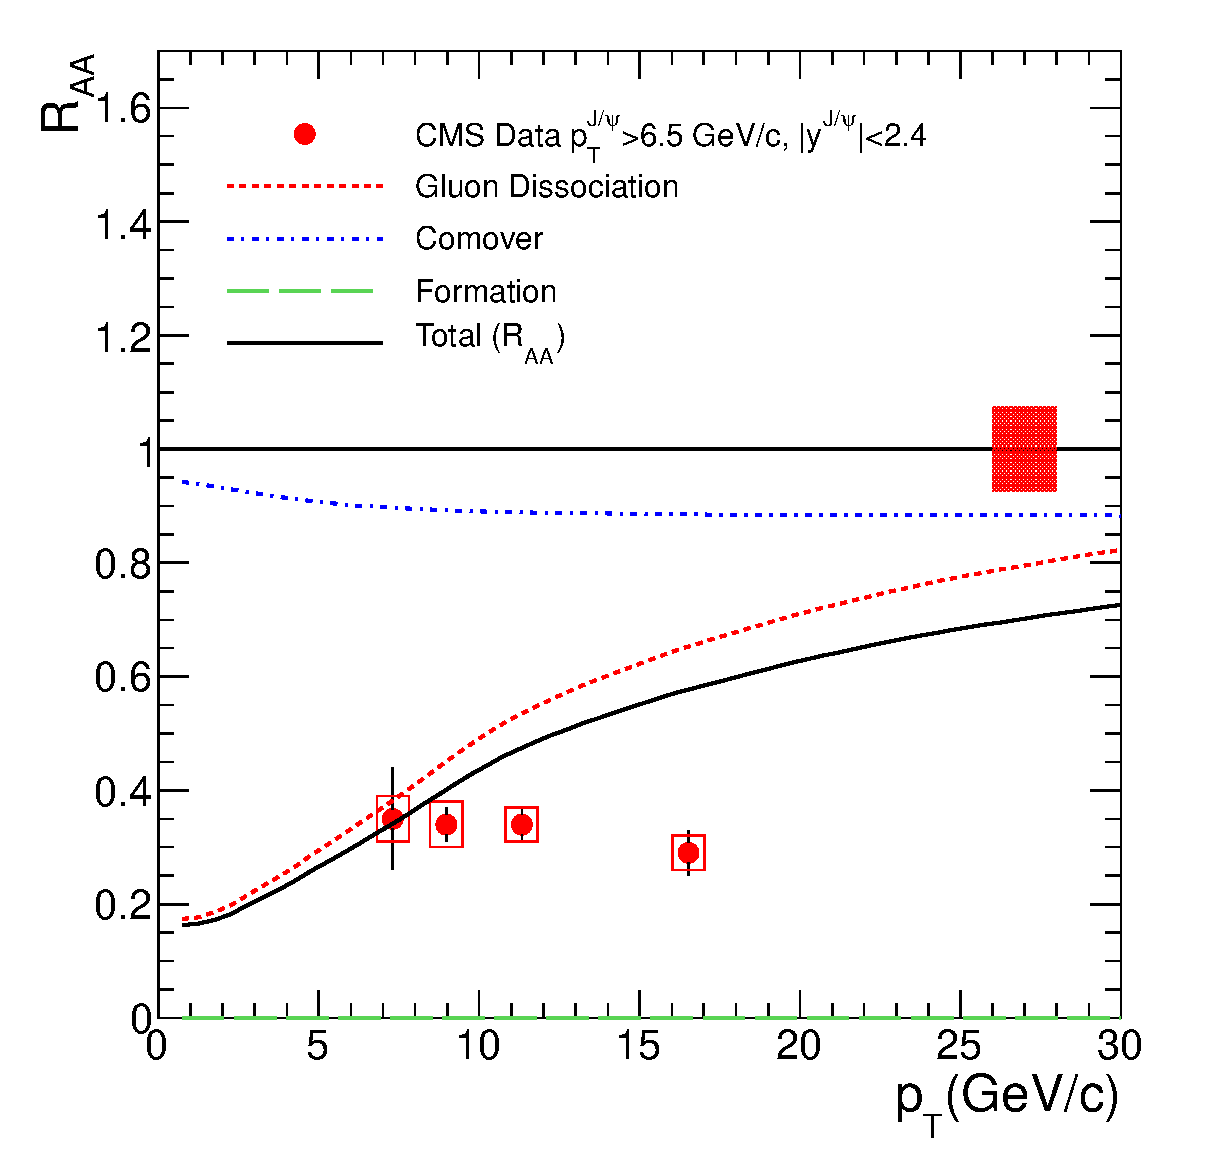
\includegraphics[width=0.49\textwidth]{Figures/Fig5b_CMS_RAAPt.eps}
\caption{(Color online) Calculated nuclear modification factor (R$_{AA}$) as a function of $\Jpsi$ 
transverse momentum compared with (a) ALICE and (b) CMS measurements.}
\label{fig:JPsiRaaVsPt}
\end{figure}


%%%%%%%%%%%%%%%%%%%%%%%%%%%%%%%%%%%%%%%%%%%%%%%%%%%%%%%%%%%%%%%%%%%%%%%%%%%%%%%%%%%%%%
%\section{Formation of quarkonia  by statistical hadronization model}\label{SHM}
% The heavy quark production at LHC is substantial which may lead to incoherent 
%recombination of uncorrelated pairs of heavy quarks and anti quarks which result 
%from multiple pair production. In statistical approach \cite{MUNZI} the number of 
%$\Jpsi$ regenrated is given by 
%\begin{eqnarray}
%N_{\Jpsi}  &= &4 {n_{ch} n_{\Jpsi} \over n_{\rm open}^2}  {N_{c\bar c}^2 \over N_{ch} }\\
%          &= &\frac{N_{c\overline{c}}^{2}}{V}\frac{4n_{\Jpsi}}{n_{open}^{2}}.
%\end{eqnarray}
%where $n_i$'s are the thermal densities, $N_{c\bar c}$ is the number of charm pairs produced 
%and $N_{ch}$ is the number of total charged particle produced. 
%The freeze out parameters are $T=170$ MeV and $\mu_B = 0$. For
%$dN_{ch}/dy = 1600$ \cite{MULT} and $dN_{c \bar c} /dy = 14.0$, we obtain $dN_{\Jpsi} /dy = 0.0092$.


\begin{figure}
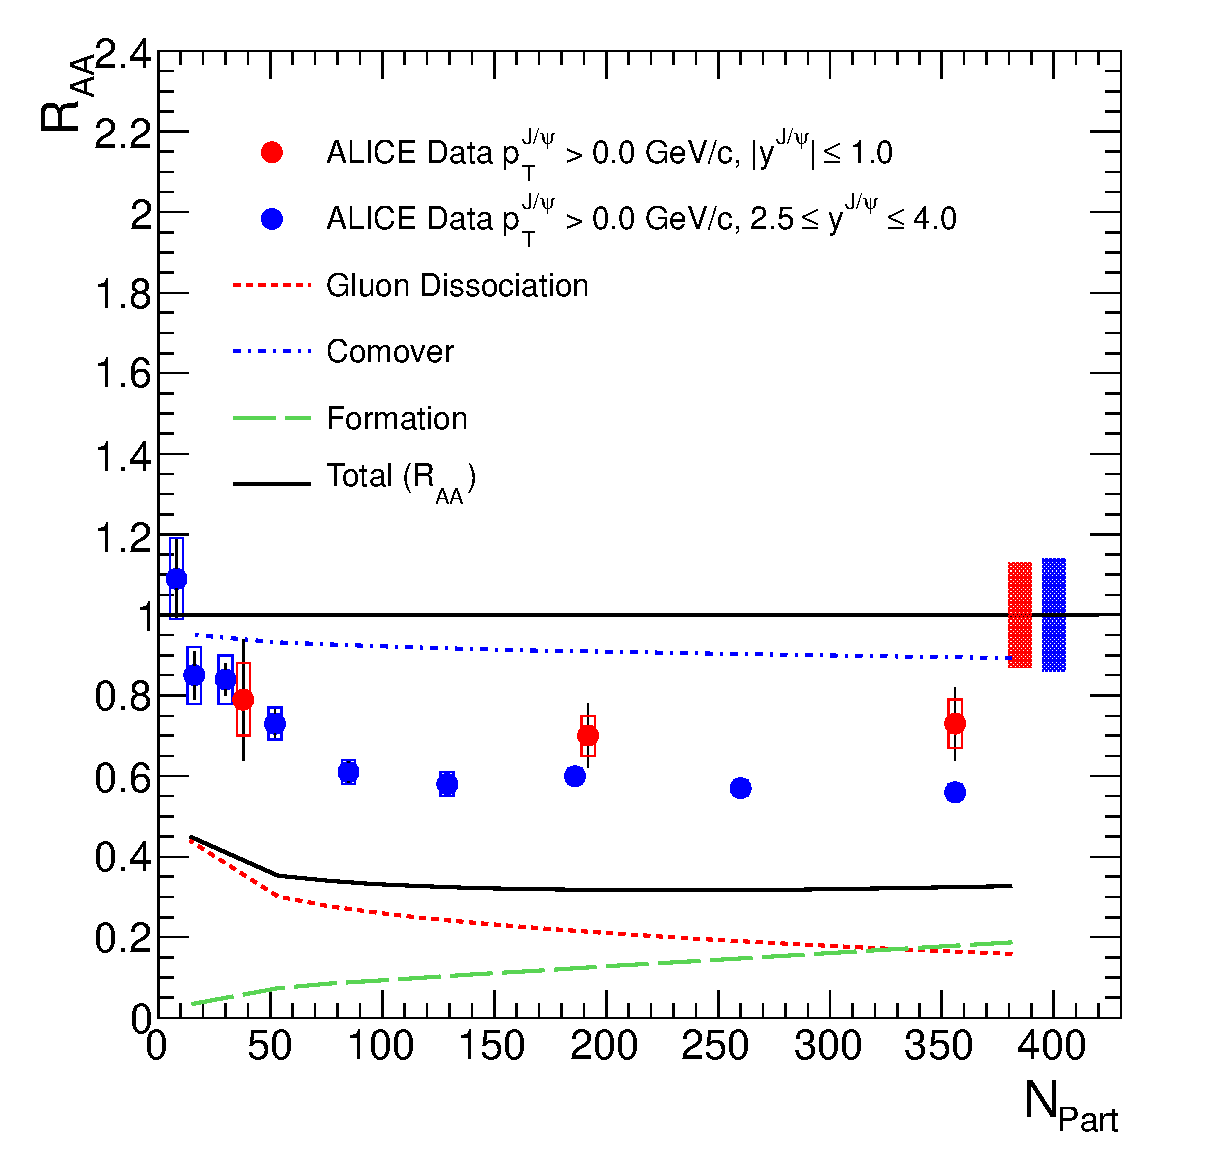
\includegraphics[width=0.49\textwidth]{Figures/Fig6a_ALICE_RAANPart.eps}
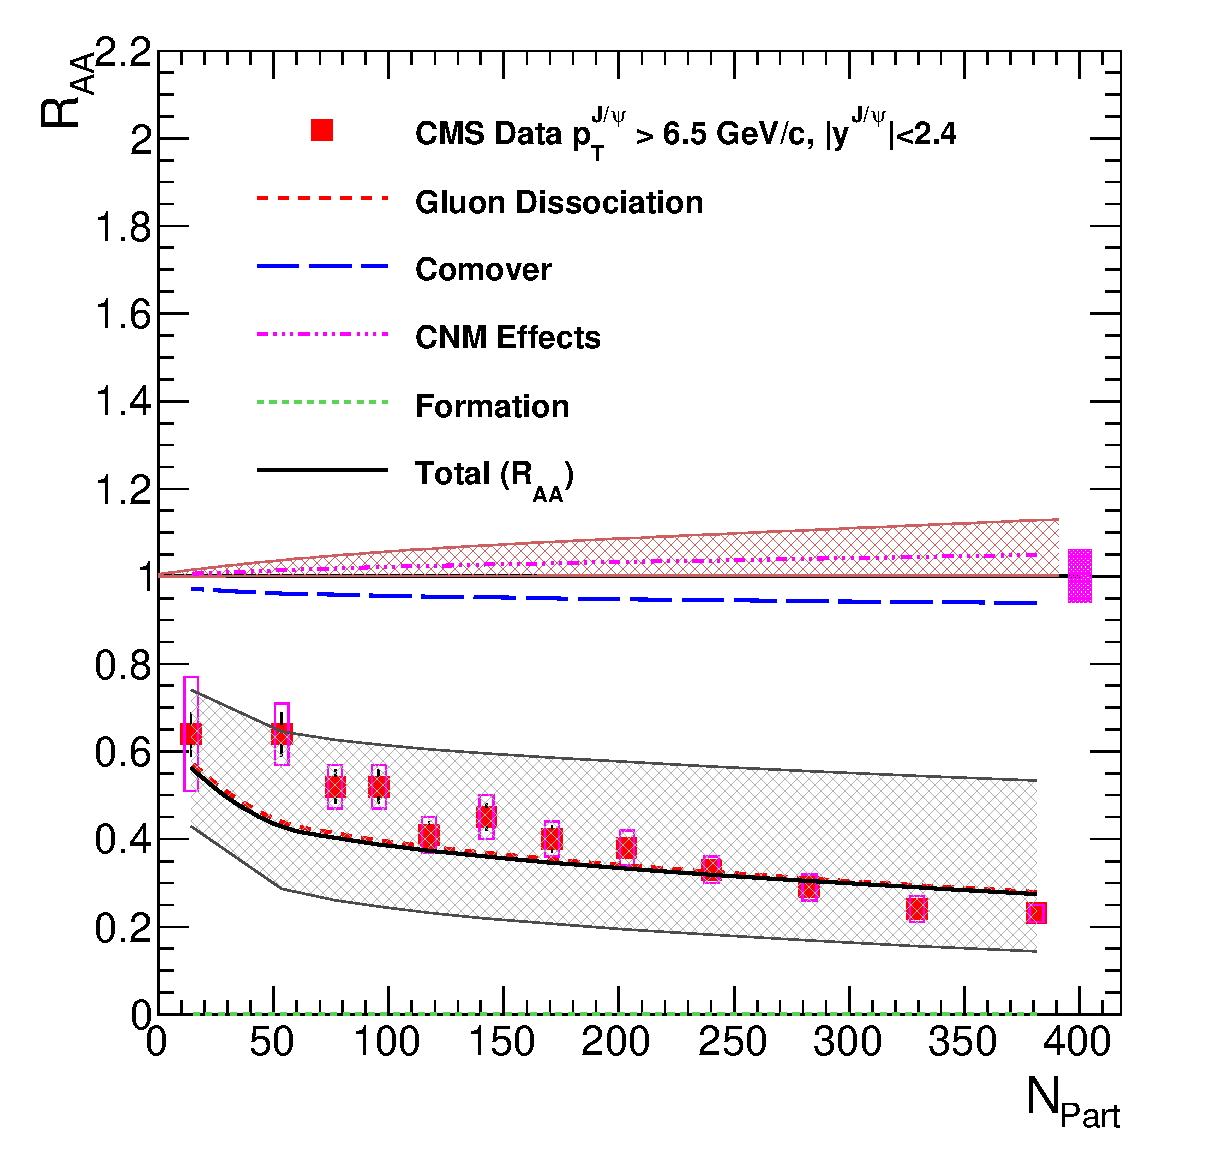
\includegraphics[width=0.49\textwidth]{Figures/Fig6b_CMS_RAANPart.eps}
%\caption{(Color online) Calculated nuclear modification factor (R$_{AA}$) compared with ALICE and CMS measurements at LHC. No regeneration is 
%considered for high p$_{T}$ CMS data. We assume similar cold nuclear matter effects for both ALICE and CMS rapidity ranges.}
\caption{(Color online) Calculated nuclear modification factor (R$_{AA}$) compared with (a) ALICE and 
(b) CMS measurements at LHC. The regeneration for high p$_{T}$ CMS comparison is negligible. 
Similar cold nuclear matter effects are assumed for both ALICE and CMS rapidity ranges.}
\label{fig:JPsiRaa}
\end{figure}


\begin{figure}
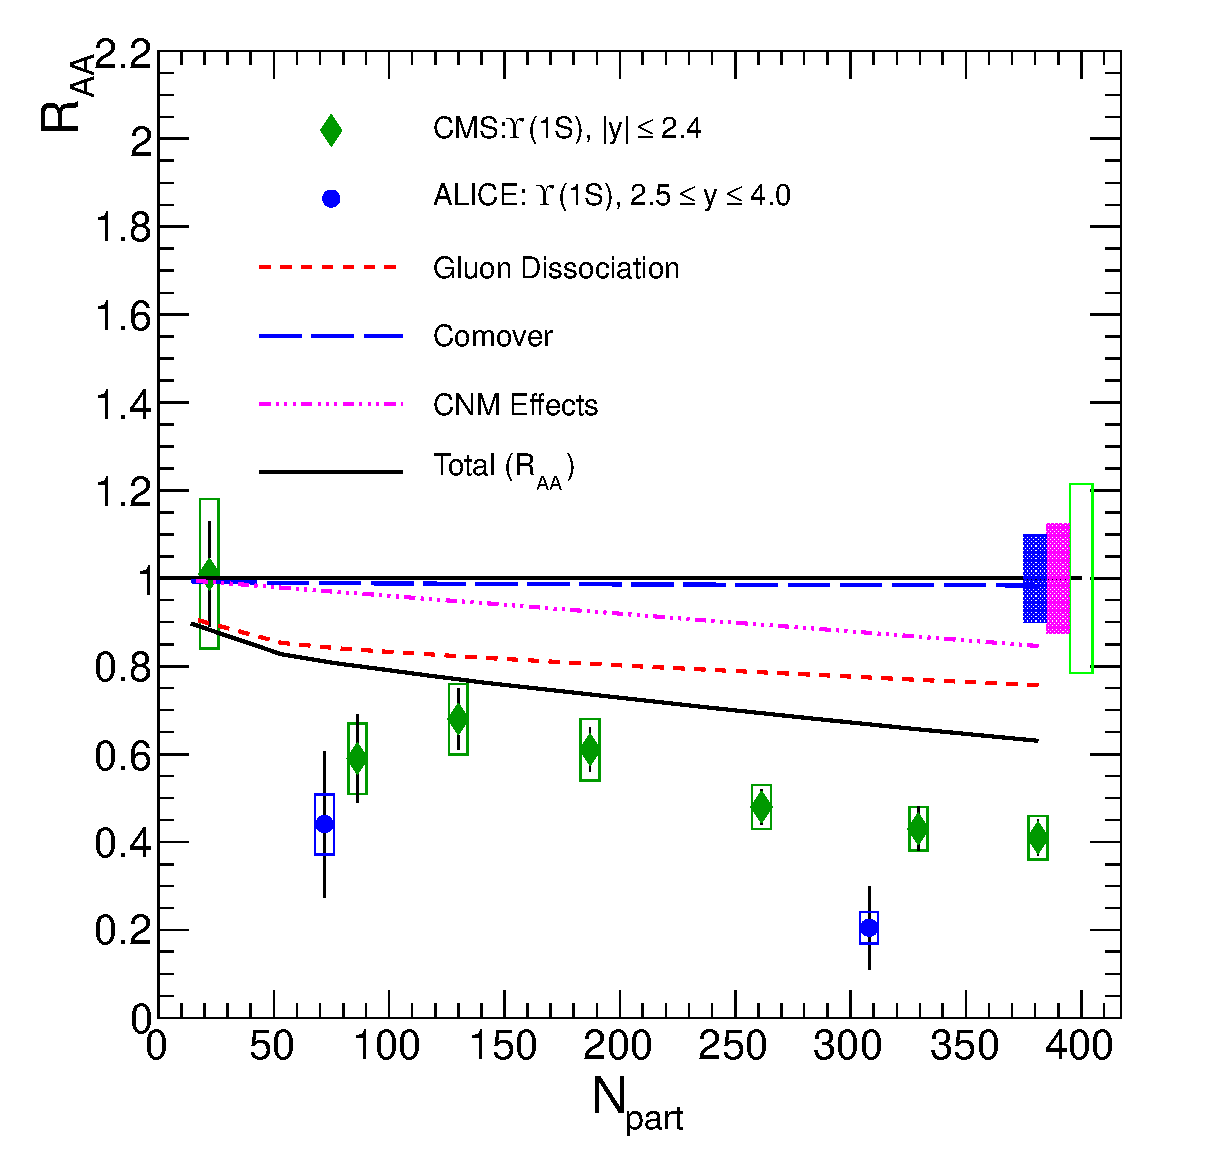
\includegraphics[width=0.49\textwidth]{Figures/Fig7a_CMS_Y1SRAANPart.eps}
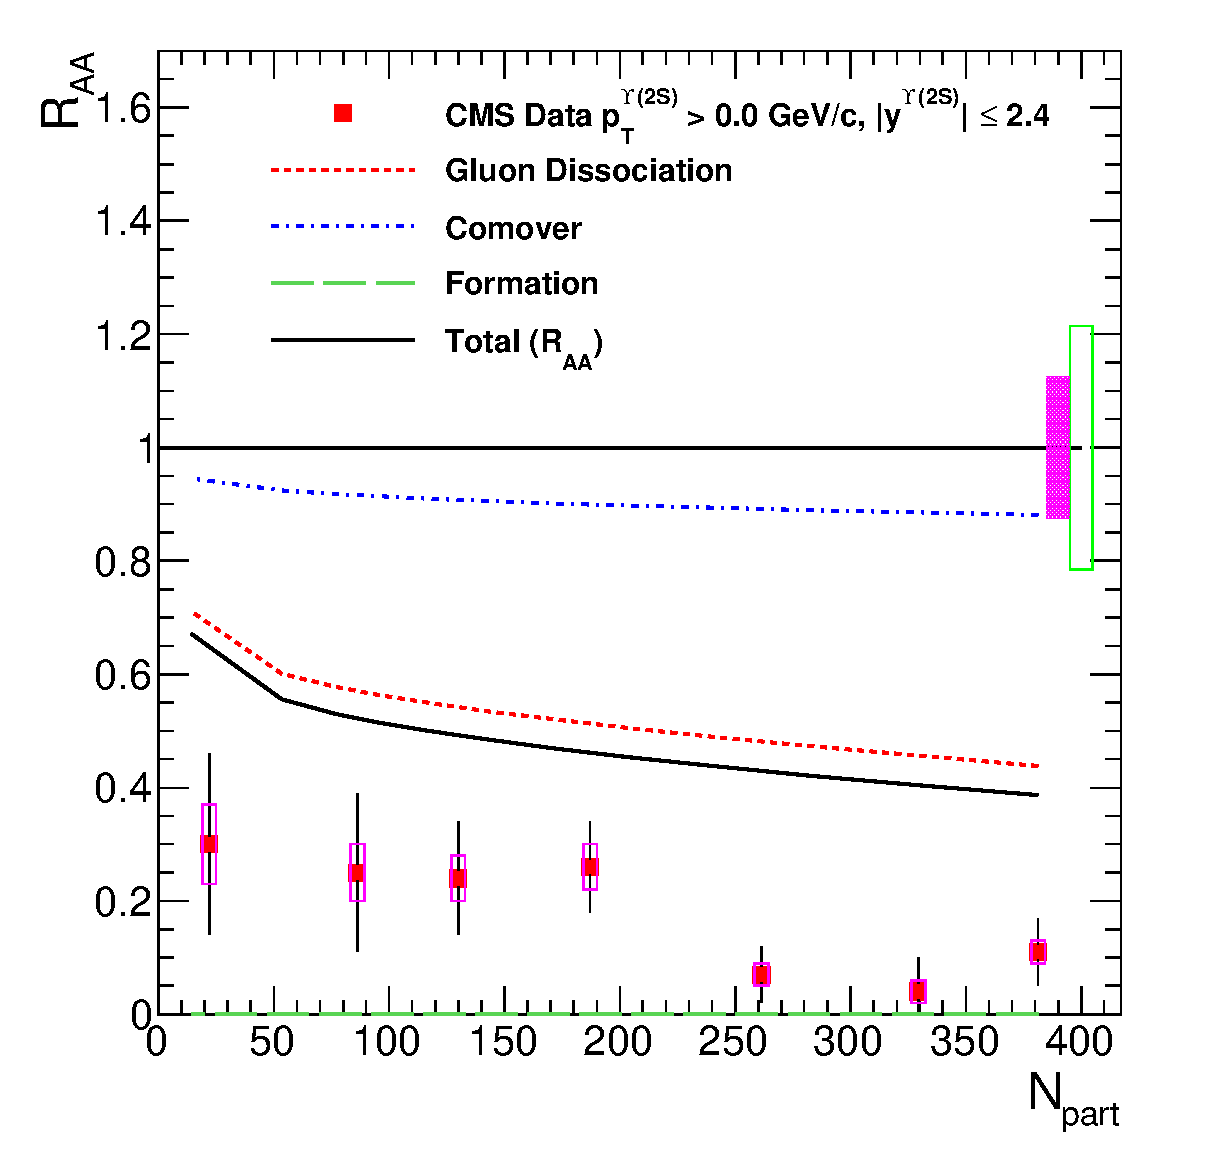
\includegraphics[width=0.49\textwidth]{Figures/Fig7b_CMS_Y2SRAANPart.eps}
%\caption{(Color online) Calculated nuclear modification factor (R$_{AA}$) compared with CMS $\Upsilon$(1S) and $\Upsilon$(2S) measurements.
%We assume small cold nuclear matter suppression than J$\psi$ and no regeneration due to small production cross section of beauty quark as shown in Table~\ref{NLOcros}.}
\caption{(Color online) Calculated nuclear modification factor (R$_{AA}$) compared with CMS 
(a) $\Upsilon$(1S) and (b) $\Upsilon$(2S) measurements.
 We assume small cold nuclear matter suppression than J$\psi$ and no regeneration due to small 
production cross section of beauty quark as shown in Table~\ref{NLOcros}.}
\label{fig:UpsilonRaa}
\end{figure}




%%%%%%%%%%%%%%%%%%%%%%%%%%%%%%%%%%%%%%%%%%%%%%%%%%%%%%%%%%%%%%%%%%%%%%%%%%%%%%%%%%%%%%%%
\section{Effect of hadronic comovers}
%The quarkonia can be suppressed due to cold matter effects such as shadowing and due to hadronic
%and comover interaction. For simplicity we approximate the combination of all CNM effects 
%by a suppression factor \cite{Rapp1,Rapp2},
%\begin{equation}
%  S_{Nucl}=\exp[-\rho_{N}\sigma_{abs}L(b)]
%  \label{CNMF}
%\end{equation}
%with an effective nuclear absorption cross section, $\sigma_{abs}$.
%We take absorption cross section, $\sigma_{abs}$ = 1.5 mb (1.5 mb) for
%$\Jpsi$($\Upsilon$). The other parameters in Eq. \ref{CNMF} are the nuclear density,
%$\rho_N$=0.14 fm$^{-3}$, and the impact-parameter dependent path length, L(b), evaluated 
%with a Glauber model \cite{GM_PShukla} for the nuclear overlap.
  The suppression of quarkonia by comoving pions can be calculated by folding the quarkonium-pion
dissociation cross section $\sigma_{\rm I}$ over thermal pion distributions \cite{Vogt:1988fj}. 
It is expected  that at LHC energies cross-section of comover suppression will be small \cite{Lourenco:2008sk}.
We take 1 mb cross-section for both $\Jpsi$ and $\Upsilon$ states.  
The dissociation rate $\lambda_{D_{\pi}}$  can be written as
\begin{eqnarray}
\lambda_{D_{\pi}} \, \rho_{\pi} & = & \frac{g_\pi}{(2\pi)^{3}} \int d^{3}p f_{\pi}(p) \sigma_{I} v_{\rm rel} \\ \nonumber
                   & = &\frac{g_\pi}{(2\pi)^{3}} \int  2\pi p^{2} dp f_{\pi}(p) \int \sigma_{\rm I} v_{\rm rel}(s) \Theta(s-4m_{D}^{2}) d(cos\theta) \\\nonumber
\end{eqnarray}
where $f_{\pi}(p,T)$ is taken as the thermal pion distribution and the  pion density $\rho_{\pi}$ is given by 
\begin{eqnarray}
\rho_\pi =\frac{g_\pi}{(2\pi)^{3}} \int d^3p \, f_{\pi}(p) 
\end{eqnarray}

The survival probability from pion collisions at freeze-out time $\tau_f$ is written as
\begin{equation}
S_\pi(p_T) = \exp \left( {-\int_{\tau_0}^{\tau_f} (1-f(\tau)) \lambda_{D_{\pi}}(T,p_T)\,\rho_{\pi}(T)\,d\tau} \right).
\end{equation}
The temperature $T(\tau)$ and the hadronic fraction (1-$f(\tau)$) 
evolve from phase transition time to freeze-out time.
The probability $S_\pi(p_T)$ is used along with $S(p_T)$ term in Eq.~(\ref{raa}).


\section{Results and discussion}
  Figure~\ref{fig:JPsiRaaVsPt}(a) show different contributions in nuclear modification factor 
($R_{AA}$) of $\Jpsi$ as a function of transverse momentum compared with ALICE measurements
\cite{Abelev:2013ila} and the Fig.~\ref{fig:JPsiRaaVsPt}(b) shows the same along with
high $p_T$ measurements of CMS experiment \cite{Mironov:2013jaa}. 
  At low $p_T$, regeneration of $\Jpsi$ is the dominant process and this seems to be the process
for the enhancement of $\Jpsi$ in the ALICE low $p_T$ data.
  The gluon suppression is also more at low $p_T$ and it reduces as we move to high $p_T$. 
Both of these processes (regeneration and dissociation) due to the presence of QGP are 
at play low and intermediate $p_T$. The high $p_T$ suppression ($p_T > 10$  GeV/$c$) of $\Jpsi$ 
measured by CMS does not seem to be originating due to dissociation by gluons in QGP.

  We have also calculated $R_{AA}$ as a function of system size.
 Figure~\ref{fig:JPsiRaa} (a) shows different contributions of $\Jpsi$ 
nuclear modification factor as a function of system size along with the measurements 
by ALICE \cite{Abelev:2013ila}.
  Figure~\ref{fig:JPsiRaa} (b) shows the same for $p_{T}\,\geq$ 6.5 GeV/c, measured 
by CMS experiment \cite{Mironov:2013jaa}. 
 From Fig.~\ref{fig:JPsiRaa} (a) indicates that  $\Jpsi$'s are increasingly suppressed 
when system size grows. Since the number of regenerated   $\Jpsi$'s also grow the nuclear 
modification factor remains flat for most of the centrality regions. Our model calculations
overestimate the suppression in the most peripheral data.
 The centrality dependence of $R_{AA}$ of $\Jpsi$ by CMS is well described by the model.
 Most of the contribution to CMS data comes from $\Jpsi$ $p_T$ between 6.5 and 10 GeV/$c$ where 
the suppression seems to be due to gluon dissociation process.


  Figure~\ref{fig:UpsilonRaa} (a) demonstrates contribution of different processes in the 
centrality dependence of $\Upsilon(1S)$ nuclear modification factor alongwith the data
measured in mid rapidity by CMS experiment\cite{Chatrchyan:2012lxa} and in forward rapidity 
by ALICE experiment \cite{Abelev:2014nua}. 
  The calculations underestimate the suppression but reproduce the shape of centrality dependence.
Figure~\ref{fig:UpsilonRaa} (b) shows the same for $\Upsilon(2S)$ nuclear modification factor
along with the measurements in mid rapidity by CMS experiment. The excited $\Upsilon(2S)$ states 
are highly suppressed .
 The effect of regeneration (not shown here) is negligible for $\Upsilon$ states.




%%%%%%%%%%%%%%%%%%%%%%%%%%%%%%%%%%%%%%%%%%%%%%%%%%%%%%%%%%%%%%%%%%%%%%%%%%%%%%%%%%%%%%%

\section{Summary}
 We have carried out detailed calculations of $\Jpsi$ and $\Upsilon$ 
modifications in PbPb collisions at LHC.
  The quarkonia and heavy flavour cross sections calculated upto NLO are used in the study 
and shadowing corrections are obtained by EPS09 parameterization.
 A kinetic model is employed which incorporates quarkonia suppression inside QGP, suppression 
due to hadronic comovers and regeneration from charm pairs.
  Their suppression is estimated using process of gluon dissociation in medium. 
The rate of regeneration has been obtained using principle of detailed balance.
  The dissociation and formation rates have been studied as a function of medium temperature
and transverse momentum of particles.
 In addition, the modification in quakonia yields due to collisions with hadronic comovers
has been estimated assuming it to be caused by pion.  

  The nuclear modification factor as a function of centrality and transverse momentum has been 
calculated  and compared to $\Jpsi$ and $\Upsilon$ nuclear modification factors measured in 
PbPb collisions at $\sqrt s_{NN}$ =  2.76 TeV.
  At low $p_T$, regeneration of $\Jpsi$ is the dominant process and this seems to be the process
for the enhancement of $\Jpsi$ in the ALICE low $p_T$ data.
  The gluon suppression is also more at low $p_T$ and it reduces as we move to high $p_T$. 
Both of these processes (regeneration and dissociation) due to the presence of QGP are 
at play low and intermediate $p_T$. The high $p_T$ suppression ($p_T > 10$  GeV/$c$) of $\Jpsi$ 
measured by CMS does not seem to be originating due to dissociation by gluons in QGP.

  The centrality dpendence of nuclear modification indicates that  $\Jpsi$'s are increasingly 
suppressed  when system size grows. Since the number of regenerated   $\Jpsi$'s also grow the nuclear 
modification factor in case of low $p_T$ measurements remains flat for most of the centrality regions. 
 The centrality dependence of $R_{AA}$ of high $p_T$ $\Jpsi$ is also well described by the model.
  The centrality dependence of suppression of $\Upsilon$ states are reproduced
by model calculations.



\section{Acknowledgement}
 The authors VK and PS thank their CMS colleagues for the fruitful discussions and comments.

\noindent
\begin{thebibliography}{100}
\medskip

\bibitem{Matsui:1986dk} 
 T.~Matsui and H.~Satz,
 ``$J/\psi$ Suppression by Quark-Gluon Plasma Formation'',
 Phys.\ Lett.\ B {\bf 178}, 416 (1986).

\bibitem{Schukraft:2013wba} 
  J.~Schukraft,
  ``Heavy Ion Physics at the LHC: What's new ? What's next ?'',
  arXiv:1311.1429 [hep-ex].

\bibitem{Kluberg:2009wc} 
  L.~Kluberg and H.~Satz,
  ``Color Deconfinement and Charmonium Production in Nuclear Collisions,''
  arXiv:0901.3831 [hep-ph].

\bibitem{Brambilla:2010cs} 
  N.~Brambilla, S.~Eidelman, B.~K.~Heltsley, R.~Vogt, G.~T.~Bodwin, E.~Eichten, A.~D.~Frawley and A.~B.~Meyer {\it et al.},
  ``Heavy quarkonium: progress, puzzles, and opportunities,''
  Eur.\ Phys.\ J.\ C {\bf 71}, 1534 (2011)
  [arXiv:1010.5827 [hep-ph]].

\bibitem{Adare:2011yf} 
  A.~Adare {\it et al.}  [PHENIX Collaboration],
  ``$J/\psi$ suppression at forward rapidity in Au+Au collisions at $\sqrt{s_{NN}}=200$ GeV,''
  Phys.\ Rev.\ C {\bf 84}, 054912 (2011)
  [arXiv:1103.6269 [nucl-ex]].

\bibitem{Andronic:2003zv} 
  A.~Andronic, P.~Braun-Munzinger, K.~Redlich and J.~Stachel,
  ``Statistical hadronization of charm in heavy ion collisions at SPS, RHIC and LHC,''
  Phys.\ Lett.\ B {\bf 571}, 36 (2003)
  [nucl-th/0303036].

\bibitem{Muller:2012zq} 
  B.~Muller, J.~Schukraft and B.~Wyslouch,
  ``First Results from Pb+Pb collisions at the LHC,''
  Ann.\ Rev.\ Nucl.\ Part.\ Sci.\  {\bf 62}, 361 (2012)
  [arXiv:1202.3233 [hep-ex]].

\bibitem{P.ShuklaforCMS:2014vna} 
  P.~Shukla [CMS Collaboration],
  ``Overview of quarkonia and heavy flavour measurements by CMS,''
  arXiv:1405.3810 [nucl-ex].

\bibitem{Chatrchyan:2012np} 
  S.~Chatrchyan {\it et al.}  [CMS Collaboration],
  ``Suppression of non-prompt $J/\psi$, prompt $J/\psi$, and Y(1S) in PbPb collisions at $\sqrt{s_{NN}}=2.76$ TeV,''
  JHEP {\bf 1205}, 063 (2012)
  [arXiv:1201.5069 [nucl-ex]].

\bibitem{Mironov:2013jaa} 
  C.~Mironov [CMS Collaboration],
  ``Overview of results on heavy flavour and quarkonia from the CMS Collaboration,''
  Nucl.\ Phys.\ A {\bf 904-905}, 194c (2013).

\bibitem{Tang:2011kr} 
  Z.~Tang [STAR Collaboration],
  ``$J/\psi$ production and correlation in p+p and Au+Au collisions at STAR,''
  J.\ Phys.\ G {\bf 38}, 124107 (2011)
  [arXiv:1107.0532 [hep-ex]].

\bibitem{Abelev:2013ila} 
  B.~B.~Abelev {\it et al.}  [ALICE Collaboration],
  ``Centrality, rapidity and transverse momentum dependence of J/$\psi$ suppression in Pb-Pb collisions at $\sqrt{s_{NN}}$=2.76 TeV,''
  Phys.\ Lett.\  {\bf 743}, 314 (2014)
  [arXiv:1311.0214 [nucl-ex]].

\bibitem{Chatrchyan:2011pe} 
  S.~Chatrchyan {\it et al.}  [CMS Collaboration],
  ``Indications of suppression of excited $\Upsilon$ states in PbPb collisions at $\sqrt{S_{NN}}$ = 2.76 TeV,''
  Phys.\ Rev.\ Lett.\  {\bf 107}, 052302 (2011)
  [arXiv:1105.4894 [nucl-ex]].

\bibitem{Chatrchyan:2012lxa} 
  S.~Chatrchyan {\it et al.}  [CMS Collaboration],
  ``Observation of sequential Upsilon suppression in PbPb collisions,''
  Phys.\ Rev.\ Lett.\  {\bf 109}, 222301 (2012)
  [arXiv:1208.2826 [nucl-ex]].

\bibitem{Abdulsalam:2012bw} 
  A.~Abdulsalam and P.~Shukla,
  ``Suppression of bottomonia states in finite size quark gluon plasma in PbPb collisions at Large Hadron Collider,''
  Int.\ J.\ Mod.\ Phys.\ A {\bf 28}, 1350105 (2013)
  [arXiv:1210.7584 [hep-ph]].

\bibitem{Bhanot:1979vb} 
  G.~Bhanot and M.~E.~Peskin,
  ``Short Distance Analysis for Heavy Quark Systems. 2. Applications,''
  Nucl.\ Phys.\ B {\bf 156}, 391 (1979).

\bibitem{Xu:1995eb} 
  X.~-M.~Xu, D.~Kharzeev, H.~Satz and X.~-N.~Wang,
  ``J/$\psi$ suppression in an equilibrating parton plasma,''
  Phys.\ Rev.\ C {\bf 53}, 3051 (1996)
  [hep-ph/9511331].

\bibitem{Andronic:2012dm} 
  A.~Andronic, P.~Braun-Munzinger, K.~Redlich and J.~Stachel,
  ``The statistical model in Pb-Pb collisions at the LHC,''
  Nucl.\ Phys.\ A {\bf 904-905}, 535c (2013)
  [arXiv:1210.7724 [nucl-th]].

\bibitem{Thews:2000rj} 
  R.~L.~Thews, M.~Schroedter and J.~Rafelski,
  ``Enhanced $J/\psi$ production in deconfined quark matter,''
  Phys.\ Rev.\ C {\bf 63}, 054905 (2001)
  [hep-ph/0007323].

\bibitem{Vogt:2010aa} 
  R.~Vogt,
  ``Cold Nuclear Matter Effects on $J/\psi$ and $\Upsilon$ Production at the LHC,''
  Phys.\ Rev.\ C {\bf 81}, 044903 (2010)
  [arXiv:1003.3497 [hep-ph]].

\bibitem{Zhao:2011cv} 
  X.~Zhao and R.~Rapp,
  ``Medium Modifications and Production of Charmonia at LHC,''
  Nucl.\ Phys.\ A {\bf 859}, 114 (2011)
  [arXiv:1102.2194 [hep-ph]].

\bibitem{Emerick:2011xu} 
  A.~Emerick, X.~Zhao and R.~Rapp,
  ``Bottomonia in the Quark-Gluon Plasma and their Production at RHIC and LHC,''
  Eur.\ Phys.\ J.\ A {\bf 48}, 72 (2012)
  [arXiv:1111.6537 [hep-ph]].

\bibitem{Pumplin:2002vw} 
  J.~Pumplin, D.~R.~Stump, J.~Huston, H.~L.~Lai, P.~M.~Nadolsky and W.~K.~Tung,
  ``New generation of parton distributions with uncertainties from global QCD analysis,''
  JHEP {\bf 0207}, 012 (2002)
  [hep-ph/0201195].

\bibitem{Pumplin:2000vx} 
  J.~Pumplin, D.~R.~Stump and W.~K.~Tung,
  ``Multivariate fitting and the error matrix in global analysis of data,''
  Phys.\ Rev.\ D {\bf 65}, 014011 (2001)
  [hep-ph/0008191].

\bibitem{Eskola:2009uj} 
  K.~J.~Eskola, H.~Paukkunen and C.~A.~Salgado,
  ``EPS09: A New Generation of NLO and LO Nuclear Parton Distribution Functions,''
  JHEP {\bf 0904}, 065 (2009)
  [arXiv:0902.4154 [hep-ph]].

\bibitem{Cacciari:2005rk} 
  M.~Cacciari, P.~Nason and R.~Vogt,
  ``QCD predictions for charm and bottom production at RHIC,''
  Phys.\ Rev.\ Lett.\  {\bf 95}, 122001 (2005)
  [hep-ph/0502203].

\bibitem{Mangano:1991jk} 
  M.~L.~Mangano, P.~Nason and G.~Ridolfi,
  ``Heavy quark correlations in hadron collisions at next-to-leading order,''
  Nucl.\ Phys.\ B {\bf 373}, 295 (1992).

\bibitem{Kumar:2012qx} 
  V.~Kumar, P.~Shukla and R.~Vogt,
  ``Components of the dilepton continuum in Pb+Pb collisions at $\sqrt{s_{_{NN}}} = 2.76 $ TeV,''
  Phys.\ Rev.\ C {\bf 86}, 054907 (2012)
  [arXiv:1205.3860 [hep-ph]].

\bibitem{Chatrchyan:2011sx} 
  S.~Chatrchyan {\it et al.}  [CMS Collaboration],
  ``Observation and studies of jet quenching in PbPb collisions at nucleon-nucleon center-of-mass energy = 2.76 TeV,''
  Phys.\ Rev.\ C {\bf 84}, 024906 (2011)
  [arXiv:1102.1957 [nucl-ex]].

\bibitem{Huovinen:2009yb} 
  P.~Huovinen and P.~Petreczky,
  ``QCD Equation of State and Hadron Resonance Gas,''
  Nucl.\ Phys.\ A {\bf 837}, 26 (2010)
  [arXiv:0912.2541 [hep-ph]].

\bibitem{Aamodt:2010cz} 
  K.~Aamodt {\it et al.}  [ALICE Collaboration],
  ``Centrality dependence of the charged-particle multiplicity density at mid-rapidity in Pb-Pb collisions at $\sqrt{s_{NN}}=2.76$ TeV,''
  Phys.\ Rev.\ Lett.\  {\bf 106}, 032301 (2011)
  [arXiv:1012.1657 [nucl-ex]].
  
\bibitem{Shuryak:1992wc} 
  E.~V.~Shuryak,
  ``Two stage equilibration in high-energy heavy ion collisions,''
  Phys.\ Rev.\ Lett.\  {\bf 68}, 3270 (1992).
  
\bibitem{Karsch:1987pv} 
  F.~Karsch, M.~T.~Mehr and H.~Satz,
  ``Color Screening and Deconfinement for Bound States of Heavy Quarks,''
  Z.\ Phys.\ C {\bf 37}, 617 (1988).
  
\bibitem{Arleo:2001mp} 
  F.~Arleo, P.~B.~Gossiaux, T.~Gousset and J.~Aichelin,
  ``Heavy quarkonium hadron cross-section in QCD at leading twist,''
  Phys.\ Rev.\ D {\bf 65}, 014005 (2002)
  [hep-ph/0102095].
  
\bibitem{Thews:2005vj} 
  R.~L.~Thews and M.~L.~Mangano,
  ``Momentum spectra of charmonium produced in a quark-gluon plasma,''
  Phys.\ Rev.\ C {\bf 73}, 014904 (2006)
  [nucl-th/0505055].
  
\bibitem{Vogt:1988fj} 
  R.~Vogt, M.~Prakash, P.~Koch and T.~H.~Hansson,
  ``$J/\psi$ Interactions With Hot Hadronic Matter,''
  Phys.\ Lett.\ B {\bf 207}, 263 (1988).
  
\bibitem{Lourenco:2008sk} 
  C.~Lourenco, R.~Vogt and H.~K.~Woehri,
  ``Energy dependence of J/$\psi$ absorption in proton-nucleus collisions,''
  JHEP {\bf 0902}, 014 (2009)
  [arXiv:0901.3054 [hep-ph]].
  
 \bibitem{Abelev:2014nua} 
   B.~B.~Abelev {\it et al.}  [ALICE Collaboration],
   ``Suppression of $\Upsilon$(1S) at forward rapidity in Pb-Pb collisions at $\sqrt{s_{\rm NN}}$ = 2.76 TeV,''
   arXiv:1405.4493 [nucl-ex].
   
   

\end{thebibliography}


\end{document}



